\label{sec:derivation}

Here the mathematical models summarized in \autoref{sec:model} are derived.
While the first two sections containing the Navier--Stokes and Favre-averaged
Navier--Stokes equations are classical and straightforward, the derivations are
provided to document the few peculiar constitutive choices as well as to
unambiguously fix nomenclature.  The third section documents a new
spatiotemporal homogenization approximation by \citet{Topalian2014Spatiotemporal}.
%
Dimensional equations are employed throughout this appendix.  The final
dimensional summary in each of the following subsections is nondimensionalized
to arrive at the formulations used in the main body of the dissertation.

\section{The Governing Equations}

\subsection{Conservation Laws}

%\subsubsection{Reynolds transport theorem}
Consider a time-varying control volume $\Omega$ with surface
$\partial\!\Omega$ and unit outward normal $\hat{n}$.  For any
scalar, vector, or tensor field quantity
$T$, Leibniz' theorem states
\begin{align}
  \label{eq:rtt}
  \frac{d}{dt}\int_{\Omega(t)}T(x,t)\,dV
  &=
  \int_{\Omega}\frac{\partial\!}{\partial\!t}T\,dV
  +
  \int_{\partial\!\Omega} \hat{n}\cdot{}w T\,dA
  =
  \int_{\Omega}\frac{\partial\!}{\partial\!t}T+\nabla\cdot{}wT\,dV
\end{align}
where $w$ is the velocity of $\partial\!\Omega$.  When $\Omega$ follows
a fixed set of fluid particles, $w$ becomes the fluid velocity $u$.

%\subsubsection{Conservation of Mass}
Since mass $M=\int_{\Omega} \rho\,dV$
and mass conservation requires $\frac{d}{dt}M=0$,
\begin{align}
  0 = \frac{d}{dt}M
  = \frac{d}{dt}\int_{\Omega} \rho\,dV
  =
  \int_{\Omega}\frac{\partial\!}{\partial\!t}\rho+\nabla\cdot{}u\rho{}\,dV.
\end{align}
Because the result holds for any control volume, locally it must be true
that
\begin{align}
  \label{eq:cons_mass}
  \frac{\partial\!}{\partial\!t}\rho+\nabla\cdot\rho{}u &= 0.
\end{align}

%\subsubsection{Conservation of Momentum}
Separating total force into surface forces and body forces,
\begin{align}
  \sum{}F
  &=
     \int_{\partial\!\Omega} f_s \, dA
   + \int_{\Omega} f \, dV
  =
     \int_{\partial\!\Omega} \sigma \hat{n} \, dA
  +  \int_{\Omega} f \, dV
  =  \int_{\Omega} \nabla\cdot\sigma + f \, dV
\end{align}
where $\sigma$ is the Cauchy stress tensor.  From linear momentum
$I=\int_{\Omega} \rho{}u\,dV$ and its conservation $\frac{d}{dt}I=\sum{}F$,
\begin{align}
    \int_{\Omega}\frac{\partial\!}{\partial\!t}\rho{}u
  + \nabla\cdot(u\otimes{}\rho{}u)\,dV
&= \int_{\Omega} \nabla\cdot\sigma + f \, dV
.
\end{align}
As the control volume may be arbitrary,
\begin{align}
  \frac{\partial\!}{\partial\!t}\rho{}u + \nabla\cdot(u\otimes{}\rho{}u)
&= \nabla\cdot\sigma + f
.
\end{align}
Lastly, separating the pressure $p$ and viscous contributions $\tau$ to
the Cauchy stress tensor so that $\sigma = -p I + \tau$,
\begin{align}
\label{eq:cons_momentum}
\frac{\partial\!}{\partial\!t}\rho{}u + \nabla\cdot(u\otimes{}\rho{}u)
&= -\nabla{}p + \nabla\cdot{}\tau + f
.
\end{align}
The conservation of angular momentum implies $\sigma=\trans{\sigma}$ and
therefore $\tau=\trans{\tau}$ too.

%\subsubsection{Conservation of Energy}
Combining internal and kinetic energy into an intrinsic density $E$,
energy $\mathscr{E}$ is
\begin{align}
  \mathscr{E} &= \int_{\Omega} \rho{}E \, dV
  .
\end{align}
Treating heat input $Q$ as both a surface phenomenon described by an outward
heat flux $q_{s}$ and as a volumetric phenomenon governed by a
body heating $q_{b}$,
\begin{align}
  Q
  &=
   \int_{\Omega}\rho{}q_{b}\,dV
  -\int_{\partial\!\Omega}\hat{n}\cdot{}q_{s}\,dA
  =
    \int_{\Omega}q_{b} - \nabla\cdot{}q_{s}\,dV
  .
\end{align}
Power input $P=F\cdot{}v$ accounts for surface stress work and body
force work to give
\begin{align}
  P
  &=
    \int_{\partial\!\Omega} \sigma{}\hat{n} \cdot{} u \, dA
  + \int_{\Omega} f \cdot{} u \, dV
  = \int_{\Omega} \nabla\cdot{}\sigma{}u + f \cdot{} u \, dV
  .
\end{align}
Demanding energy conservation $\frac{d}{dt}\mathscr{E}=Q+P$,
\begin{align}
  \int_{\Omega}\frac{\partial\!}{\partial\!t} \rho{}E
  +
  \nabla\cdot{}u\rho{}E
  \,dV
&=
    \int_{\Omega} q_{b} - \nabla\cdot{}q_{s}\,dV
  + \int_{\Omega} \nabla\cdot\sigma{}u + f \cdot{} u \, dV
  .
\end{align}
Again, since the control volume was arbitrary,
\begin{align}
  \frac{\partial\!}{\partial\!t} \rho{}E
  +
  \nabla\cdot{}\rho{}Eu
&=
  - \nabla\cdot{}q_{s}
  + \nabla\cdot\sigma{}u
  + f \cdot{} u
  + q_{b}
  .
\end{align}
Splitting $\sigma$'s pressure and viscous stress contributions into separate
terms,
\begin{align}
  \label{eq:cons_energy}
  \frac{\partial\!}{\partial\!t} \rho{}E
  +
  \nabla\cdot{}\rho{}Eu
&=
  - \nabla\cdot{}q_{s}
  - \nabla\cdot{}pu
  + \nabla\cdot{}\tau{}u
  + f \cdot{} u
  + q_{b}
  .
\end{align}

\subsection{Constitutive Assumptions}
\label{sec:constitutive}

%\subsubsection{Perfect gas}

Assume the fluid is a thermally and calorically perfect gas governed by
\begin{align}
  \label{eq:perfectgaseos}
  p &= \rho{} R T
\end{align}
where $R$ is the gas constant. The constant volume $C_{v}$ specific heat,
constant pressure specific heat $C_{p}$, and acoustic velocity $a$
relationships follow:
\begin{align}
  \label{eq:perfectgasrelations}
  \gamma &= \frac{C_{p}}{C_{v}}
  &
  C_{v} &= \frac{R}{\gamma - 1}
  &
  C_{p} &= \frac{\gamma{}R}{\gamma-1}
  &
  R &= C_{p} - C_{v}
  &
  a^{2} = \gamma{}RT.
\end{align}
Also assume $C_{v}$ and $C_{p}$ and, therefore, $\gamma$ are constant.
The total (internal and kinetic) energy density is
\begin{align}
  \label{eq:perfectgastotalenergy}
  E &= C_{v} T + \frac{1}{2}u^{2}
     = \frac{RT}{\gamma-1} + \frac{1}{2}u^{2}
\end{align}
where the notation $u^2 = u\cdot{}u$ is employed.
The total enthalpy density $H$ and (internal) enthalpy density $h$ are
\begin{align}
  \label{eq:perfectgasenthalpy}
  H &= E + \frac{p}{\rho}
     = C_{p} T + \frac{1}{2}u^{2}
     = \frac{\gamma{}RT}{\gamma-1} + \frac{1}{2}u^{2},
\\
  h &= H - \frac{1}{2}u^{2}
     = C_{p} T
     = \frac{\gamma{}RT}{\gamma-1}
  .
\end{align}
See a gas dynamics reference, for example \citet{LiepmannRoshko2002}, for more
details.

%\subsubsection{Newtonian fluid}
\label{sec:newtonianfluid}

If one seeks a constitutive law for the viscous stress tensor $\tau$
using only velocity information, the principle of material frame
indifference implies that uniform translation (given by velocity $u$)
and solid-body rotation (given by the skew-symmetric rotation tensor
$\omega=\frac{1}{2}\left( \nabla{}u-\trans{\nabla{}u} \right)$)
may not influence $\tau$.  Considering contributions only up to the
gradient of velocity, extensional strain (dilatation) and shear strain
effects may depend on only the symmetric strain rate tensor
$\varepsilon=\frac{1}{2}\left( \nabla{}u+\trans{\nabla{}u}\right)$
and its principal invariants.

Assuming $\tau$ is isotropic and depends linearly upon only $\varepsilon$,
express it as
\begin{align}
\tau_{ij}
&= c_{ijmn} \varepsilon_{mn}
\notag \\
&= \left( A \delta_{ij} \delta_{mn}
        + B \delta_{im} \delta_{jn}
        + C \delta_{in} \delta_{jm}
    \right) \varepsilon_{mn}
&
&\text{for some }A, B, C\in\mathbb{R}
\notag \\
&= A \delta_{ij} \varepsilon_{mm} + B\varepsilon_{ij} + C\varepsilon_{ji}
\notag \\
&= A \delta_{ij} \varepsilon_{mm} + \left( B+C \right)\varepsilon_{ji}
\notag \\
&= 2 \mu \varepsilon_{ij} + \lambda\delta_{ij}\nabla\cdot{}u
\end{align}
where $\mu=\frac{1}{2}\left( B + C \right)$ is the dynamic coefficient of
viscosity (shear) and $\lambda=A$ is the second coefficient of viscosity
(dilatational).  Reverting to direct notation,
\begin{align}
\tau
&= 2 \mu \varepsilon + \lambda \left( \nabla\cdot{}u \right) I
\label{eq:taunewt}
 =   \mu \left( \nabla{}u + \trans{\nabla{}u} \right)
   + \lambda \left( \nabla\cdot{}u \right) I
.
\end{align}

The bulk viscosity $\mu_{B}=\lambda + \frac{2}{3}\mu$ and the deviatoric
part of the strain rate tensor,
\begin{align}
  S &= \varepsilon - \frac{1}{3} \trace\left(\varepsilon\right) I
     = \frac{1}{2}\left(\nabla{}u + \trans{\nabla{}u}\right)
     - \frac{1}{3}\left(\nabla\cdot{}u\right)I,
\end{align}
may be used to write
\begin{align}
\label{eq:tauSmub}
  \tau &= 2 \mu S + \mu_B  \left( \nabla\cdot{}u \right) I
.
\end{align}
The kinematic viscosity and bulk kinematic viscosity
\begin{align}
 \nu &= \frac{\mu}{\rho} & \nu_{B} &= \frac{\mu_{B}}{\rho}
\end{align}
are often used to simplify notation.

%\subsubsection{Stokes' hypothesis}
\label{sec:stokeshypothesis}

Set the bulk viscosity $\mu_{B}$ to be a fixed multiple of the dynamic
viscosity $\mu$.  This relationship may be written as either
\begin{align}
\label{eq:secondviscosityclaw}
\mu_{B} &= \alpha \mu
&
&\text{or}
&
\lambda &= \left( \alpha - \frac{2}{3} \right) \mu
\end{align}
where a dimensionless proportionality constant $\alpha$ has been introduced.
Stokes' hypothesis that bulk viscosity is negligible may be recovered by
selecting $\alpha = 0$.  Though Stokes' hypothesis is valid for most
circumstances~\citep{GadelHak1995}, we choose to separately track $\mu$ and
$\lambda$ terms in the model.

%\subsubsection{Power Law Viscosity}

Assume that viscosity varies only with temperature according to
\begin{align}
\label{eq:powerlawviscosity}
\frac{\mu}{\mu_{0}}=\left(\frac{T}{T_{0}}\right)^{\beta}
\end{align}
where $\mu_{0}$ and $T_{0}$ are suitable reference values.  This relationship
models air well for temperatures up to several thousand degrees
Kelvin~\citep{NASA-TR-R-132} as shown in \autoref{fig:Svehla1962}.
Sutherland's law~\citep{Sutherland1893Viscosity}, often recommended for its
greater accuracy~\citep[p. 46]{Smits2005Turbulent}, was avoided
because of the greater complexity its use would entail in expressions like
\eqref{eq:Tmonstrosity}.

\begin{figure}[tb]
\centering
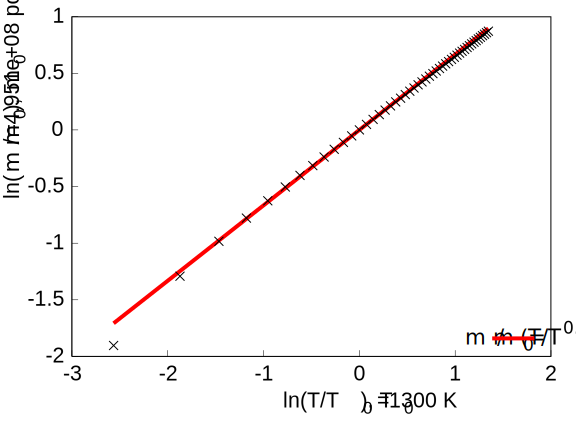
\includegraphics[height=0.6\textwidth]{AirViscosityVsTemperature}
\caption[Viscosity of air versus temperature from 100 to 5000K]{%
    Power law fit for air viscosity versus temperature over 100 to 5000 K using
    data from \citet{NASA-TR-R-132}.  The least squares fit over this wide range
    is relatively insensitive to the chosen references $\mu_0$ and $T_0$.  For
    example, selecting $T_0 = 300K$ or $4000K$ causes exponents $0.6639$ or
    $0.6673$ to be optimal, respectively.  Truncating the data to eliminate
    larger $T$ generally produces larger exponents.
\label{fig:Svehla1962}
}
\end{figure}

%\subsubsection{Fourier's Equation}

Neglecting the transport of energy by molecular diffusion and radiative heat
transfer, a linear relation is sought between the surface heat flux $q_{s}$ and
the temperature $T$.  The principle of frame indifference implies only the
temperature gradient is relevant so that
\begin{align}
  \label{eq:fouriertensorlaw}
  q_{s} &= \underline{\kappa} \cdot \nabla{} T
\end{align}
where $\underline{\kappa}$ is a thermal conductivity tensor.
Consistent with the assumption that $\tau$ is isotropic, assume
$\underline{\kappa}$ is isotropic to obtain
\begin{align}
  \label{eq:fourierlaw}
  q_{s} &= - \kappa \nabla{} T
\end{align}
where $\kappa$ is the scalar thermal conductivity.  The negative sign has been
introduced so that heat flows from hot to cold when $\kappa>0$.

%\subsubsection{Constant Prandtl Number}

Assume the Prandtl number $\Prandtl = \mu{}C_{p}/\kappa$ is constant.
Because $C_{p}$ is constant the ratio $\mu/\kappa$ must be
constant.  The viscosity and thermal conductivity must either grow at
identical rates or they must grow according to an inverse relationship.
The latter is not observed in practice for this class of fluids, and
so further assume
\begin{align}
  \frac{\mu}{\mu_{0}} = \frac{\kappa}{\kappa_{0}}
  .
  \label{eq:mukappa}
\end{align}

\subsection{Dimensional Summary}

Combining the conservation laws with the above constitutive relations
and assumptions, one arrives at the dimensional equations
\begin{subequations}\label{eq:dimensionalmodel}
\begin{align}
  \label{eq:dim_continuity}
  \frac{\partial\!}{\partial\!t}\rho
&=
  - \nabla\cdot\rho{}u
  + \Ssd_\rho
  \\
  \label{eq:dim_momentum}
  \frac{\partial\!}{\partial\!t}\rho{}u
&=
  - \nabla\cdot(u\otimes{}\rho{}u)
  -\nabla{} p
  + \nabla\cdot{} \tau
  + f
  + \Ssd_{\rho{} u}
  \\
  \label{eq:dim_energy}
  \frac{\partial\!}{\partial\!t} \rho{}E
&=
  - \nabla\cdot{}\rho{}Eu
  + \nabla\cdot{} \frac{\kappa_{0}}{\mu_{0}} \mu \nabla{} T
  - \nabla\cdot{} p u
  + \nabla\cdot{}\tau{} u
  + f \cdot{} u
  + q_{b}
  + \Ssd_{\rho{} E}
\intertext{
  where the right hand sides make use of
}
  \label{eq:dim_pressure}
  p &=   \left(\gamma-1\right)\left(\rho{}E
       - \frac{1}{2}\rho{}u^{2} \right)
  \\
  \label{eq:dim_temperature}
  T &= \frac{p}{\rho{}R}
  \\
  \label{eq:dim_viscosity}
  \mu &= \mu_{0} \left( \frac{T}{T_{0}} \right)^{\beta}
  \\
  \label{eq:dim_secondviscosity}
  \lambda &= \left(\alpha- \frac{2}{3}\right) \mu
  \\
  \label{eq:dim_viscousstress}
  \tau &=   \mu \left( \nabla{}u + \trans{\nabla{}u} \right)
          + \lambda \left( \nabla\cdot{}u \right) I
  .
\end{align}
\end{subequations}
Additional, equation-specific terms $\Ssd_\rho$, $\Ssd_{\rho u}$, and
$\Ssd_{\rho E}$ have been added to permit applying forcing arising from
homogenization.  Appropriately nondimensionalized, these equations are nothing
but the model given in \autoref{sec:goveqn}.

\section{The Favre-Averaged Navier--Stokes Equations}

The material in this section borrows from
\citet{OliverFANSModels2011}.  It departs from that particular document in that
it employs the preceding constitutive relationships, avoids introducing
customary assumptions about the relative importance of unclosed terms, and
accounts for arbitrary slow growth forcing.

\subsection{Reynolds- and Favre-Averaging Techniques}
\label{sec:averagingtechniques}

The Reynolds average is the usual mean of a random variable.  Consider a
generic flow variable $q$.  The value, $q(x, y, z, t)$, of this variable at a
particular point in space, $(x, y, z)$, and time, $t$, is a random variable.
Assuming that the probability density function for $q(x, y, z, t)$ is given by
$\pi_q(V; x, y, z, t)$, the Reynolds average is defined by
%
\begin{equation}
\label{eqn:reynoldsAvg}
\bar{q}(x, y, z, t) \equiv \int V \pi_q(V; x, y, z, t) \,\mathrm{d} V.
\end{equation}
%
The Favre average is defined as the density-weighted average.  Thus,
denoting the fluid density by $\rho(x,y,z, t)$, the Favre average of
$q(x,y,z, t)$ is
%
\begin{equation}
\tilde{q}(x,y,z, t) \equiv \frac{ \overline{\rho q}(x,y,z, t) }{ \bar{\rho}(x,y,z, t) }.
\end{equation}
%
It is
assumed that both the Reynolds and Favre averages are well-defined for
any required flow variable, $q$.  That is, the integral on the
right-hand side of~\eqref{eqn:reynoldsAvg} exists whenever required,
and the Reynolds-averaged density, $\bar{\rho}$, is positive
everywhere.

In the following, the flow variables will be decomposed into mean and
fluctuating parts.  Specifically, the fluctuations about the
mean---denoted by $(\cdot)'$ and $(\cdot)''$ for the Reynolds and
Favre averages, respectively---are defined by the following
relationships:
%
\begin{align}
q' &\equiv q - \bar{q}, \\
q'' &\equiv q - \tilde{q}.
\end{align}
%
Using the linearity of the Reynolds average and the fact that
$\bar{q}$ and $\tilde{q}$ are deterministic,
%
\begin{gather}
\overline{q'} = \overline{q - \bar{q}} = \bar{q} - \bar{q} =  0, \\
\widetilde{q''} = \widetilde{q - \tilde{q}} = \tilde{q} - \tilde{q} = 0.
\end{gather}
%
Furthermore,
%
\begin{equation}
\overline{\rho q''} = \bar{\rho} \widetilde{q''} = 0.
\end{equation}
%
However, in general,
%
\begin{equation}
\overline{q''} = \overline{q - \tilde{q}} = \bar{q} - \tilde{q} \neq 0
\end{equation}
which proves that
the Reynolds and Favre averages differ by exactly $\overline{q''}$.

Wherever necessary, realizations of random fields of flow quantities
are assumed to be differentiable in both time and space so that Reynolds
averaging and differentiation commute.  For example,
%
\begin{equation}
\overline{ \nabla{}u } = \nabla\bar{u}.
\end{equation}
%
This commutativity is used to develop the FANS equations.  In contrast, Favre
averaging and differentiation do not, in general, commute:
\begin{align*}
  \rho \nabla q &= \rho \nabla q
\\
   \rho \widetilde{\nabla{}q} + \rho \left(\nabla{}q\right)''
&=
   \rho \nabla \tilde{q} + \rho \nabla{}q''
\\
     \bar{\rho} \widetilde{\nabla{}q}
&=
     \bar{\rho} \nabla{\tilde{q}}
   + \overline{\rho \nabla{}q''}
\\
&=
     \bar{\rho} \nabla{\tilde{q}}
   - \overline{q''\nabla\rho}.
\end{align*}
Here the common convention that taking Favre fluctuations,
$\left(\cdot\right)''$, has higher precedence than differentiation,
$\nabla\left(\cdot\right)$, has been adopted.  Rearranging to better examine
the difference between $\widetilde{\nabla{}q}$ and $\nabla\tilde{q}$ in terms
of mean quantities,
\begin{align}
  \label{eq:favremeancommute}
  \widetilde{\nabla{}q}
  -
  \nabla{\tilde{q}}
&=
  \widetilde{\nabla{}q''}
= - \frac{{\overline{q''\nabla\rho}}}{\bar{\rho}}
= \frac{\tilde{q}\nabla\bar{\rho}}{\bar{\rho}}
  - \frac{\overline{q\nabla\rho}}{\bar{\rho}}
.
\end{align}
This lack of commutativity is not problematic as it is not required to derive the
FANS equations.  It does, however, slightly complicate the mean constitutive
relationships.  The fluctuating gradient and the gradient of the fluctuations
differ according to
\begin{align}
  \label{eq:favrefluctcommute}
  \left(\nabla{}q\right)'' - \nabla{}q'' &= - \widetilde{\nabla{}q''}
.
\end{align}
In some circumstances, the difference between quantities written using a
fluctuating gradient and the gradient of the fluctuations can vanish.
One useful example is
\begin{align}
  \label{eq:favrefluctexample}
\widetilde{f''\left(\nabla{}g\right)''}
&=
\frac{\overline{\rho{}f''\left(\nabla{}g\right)''}}
     {\bar{\rho}}
=
\frac{  \overline{\rho{}f''\left(\nabla{}g''
      - \widetilde{\nabla{}g''}\right)}}
     {\bar{\rho}}
=
\frac{  \overline{\rho{}f''\nabla{}g''}
      - \overline{\rho{}f''}\widetilde{\nabla{}g''}}
     {\bar{\rho}}
=
\widetilde{f''\nabla{}g''}
.
\end{align}

\subsection{Derivation of the Favre-Averaged Equations}
\label{sec:derivation_FANS}

From~\eqref{eq:dimensionalmodel} a lengthy algebraic procedure
\citep[\textsection{}2]{OliverFANSModels2011} produces exact equations governing
the evolution of mean conserved quantities
$\bar{\rho}$, $\overline{\rho{}u}= \bar{\rho}\tilde{u}$, and
$\overline{\rho{}E} = \bar{\rho}\tilde{E}$:
\begin{subequations}\label{eq:unclosedfansequations}
\begin{align}
    \frac{\partial\!}{\partial\!t}\bar{\rho}
 =
 &- \nabla\cdot\bar{\rho}\tilde{u}
  + \overline{\Ssd_{\rho{}}}
\\
    \frac{\partial\!}{\partial\!t}\bar{\rho}\tilde{u}
 =
 &- \nabla\cdot(\tilde{u}\otimes\bar{\rho}\tilde{u})
  - \nabla{}\bar{p}
  + \nabla\cdot\left(
        \bar{\tau}
      - \bar{\rho}\widetilde{u''\otimes{}u''}
    \right)
  + \bar{f}
  + \overline{\Ssd_{\rho{} u}}
\\
  \frac{\partial\!}{\partial\!t} \bar{\rho}\tilde{E}
 =
 &- \nabla\cdot{}\bar{\rho}\tilde{H}\tilde{u}
  + \nabla\cdot\left(
        \left(
            \bar{\tau}
          - \bar{\rho} \widetilde{u''\otimes{}u''}
        \right) \tilde{u}
      - \frac{1}{2}\bar{\rho}\widetilde{{u''}^{2}u''}
      + \overline{\tau{}u''}
    \right)
\notag\\
 &- \nabla\cdot\left(
        \bar{q}_s
      + \bar{\rho} \widetilde{h''u''}
    \right)
  + \bar{f}\cdot\tilde{u}
  + \overline{f\cdot{}u''}
  + \bar{q}_{b}
  + \overline{\Ssd_{\rho{} E}}.
\end{align}
\end{subequations}
Several correlations impact the evolution of mean quantities: the Reynolds
stress $-\bar{\rho}\widetilde{u''\otimes{}u''}$, the Reynolds heat flux
$\bar{\rho} \widetilde{h''u''}$, turbulent transport
$-\frac{1}{2}\bar{\rho}\widetilde{{u''}^{2}u''}$, turbulent work
$\overline{\tau{}u''}$, and the forcing-velocity correlation
$\overline{f\cdot{}u''}$.  The Reynolds stress and heat flux augment the
viscous stress and heat flux, respectively.  The turbulent transport and work
terms represent transport of the turbulent kinetic energy density~$k$, defined
below, and viscous stress work due to turbulent velocity fluctuations,
respectively.

We now turn to perfect gas relations from \autoref{sec:constitutive}.
The Reynolds average of~\eqref{eq:perfectgaseos} gives
\begin{align}
  \bar{p} &= R\overline{\rho{}T} = \bar{\rho}R\tilde{T}
\end{align}
while the Favre average of~\eqref{eq:perfectgasenthalpy} finds both
\begin{align}
 \tilde{H} &= \tilde{E} + R \tilde{T},
&
 \tilde{h} &= \frac{\gamma{}R\tilde{T}}{\gamma-1}.
\end{align}
The turbulent kinetic energy density,
\begin{align}
  k &= \frac{1}{2}\widetilde{{u''}^2},
 \end{align}
arises from averaging the total energy given by
\eqref{eq:perfectgastotalenergy}:
\begin{align}
  \rho{} E
&=
  \frac{R}{\gamma-1} \rho{}T + \frac{1}{2}\rho{} u^{2}
\notag\\
&=
  \frac{R}{\gamma-1} \rho{}\left( \tilde{T} + T'' \right)
+ \frac{1}{2}\rho{} \left( \tilde{u} + u'' \right)^2
\\
  \overline{\rho{}E}
&=
  \frac{R}{\gamma-1} \bar{\rho} \tilde{T}
+ \frac{1}{2}\bar{\rho} \tilde{u}^2
+ \frac{1}{2}\overline{\rho{}{u''}^2}
\\
  \tilde{E}
&=
  \frac{R}{\gamma-1} \tilde{T}
+ \frac{1}{2} \tilde{u}^2
+ k.
\end{align}

An exact equation may be derived for the evolution of $k$
\citep[\textsection{}5]{OliverFANSModels2011}
\begin{align}
\label{eq:fanstke1}
    \frac{\partial\!}{\partial\!t}\bar{\rho}k
 =
 &- \nabla\cdot\bar{\rho}k\tilde{u}
  - \bar{\rho} \widetilde{u''\otimes{}u''} : \nabla\tilde{u}
  - \bar{\rho} \epsilon
  + \nabla\cdot\left(
        -\frac{1}{2}\bar{\rho}\widetilde{{u''}^{2}u''}
      + \overline{\tau{}u''}
    \right)
\notag\\
 &- \overline{u''}\cdot\nabla\bar{p}
  - \nabla\cdot\overline{p' u''}
  + \overline{p' \nabla\cdot{}u''}
  + \overline{f\cdot{}u''}
  + \overline{\Ssd_{\rho{} u}\cdot{}u''}
\end{align}
where $A:B$ denotes $\trace \left(\trans{A} B\right)$, and the contribution of
the slow growth terms has been tallied.  The dissipation rate
density $\epsilon$, which governs the conversion rate from $k$ to mean internal
energy, is defined by
\begin{align}
  \bar{\rho} \epsilon &= \overline{\tau : \nabla{}u''}.
\end{align}

Many authors, for example \citet{Guarini2000Direct}, work
with~\eqref{eq:fanstke1}.  However, a different form the turbulent kinetic
energy equation is preferred here.  As \citet[page 216]{Lele1994Compressibility}
suggests, expanding $\rho H u$ using $\rho{}H = \rho{}E + p$, decomposing the
non-density contributions into their mean and fluctuating contributions,
averaging, and then subtracting $\left(\bar{\rho}\tilde{H} = \bar{\rho}\tilde{E}
+ \bar{p}\right)\tilde{u}$ proves the general identity
\begin{align}
    \bar{\rho}\widetilde{H''u''}
    &=
    \bar{\rho}\widetilde{E''u''}
    + \bar{p}\overline{u''}
    + \overline{p'u''}.
\end{align}
Collecting $\left(H-E\right)''$, introducing perfect gas constitutive relations,
and simplifying,
\begin{align}
  \overline{u''}
&=
  \frac{\widetilde{T''u''}}{\tilde{T}} - \frac{\overline{p'u''}}{\bar{p}}.
\end{align}
Substituting $h''$ everywhere for $T''$, noting $\bar{p}/\tilde{h} =
\frac{\gamma-1}{\gamma}\bar{\rho}$, and differentiating,
\begin{align}
  \overline{p'u''}
&=
  \frac{\gamma-1}{\gamma} \bar{\rho} \widetilde{h''u''}
- \bar{p} \overline{u''}
\\
  \nabla\cdot \overline{p'u''}
&=
  \frac{\gamma-1}{\gamma} \nabla\cdot \bar{\rho} \widetilde{h''u''}
- \bar{p}\nabla\cdot\overline{u''}
- \overline{u''}\cdot\nabla{}\bar{p}
.
\end{align}
Rearranging the above result to mimic terms within~\eqref{eq:fanstke1}
\begin{align}
  - \overline{u''}\cdot\nabla\bar{p}
  - \nabla\cdot\overline{p'u''}
&=
  \bar{p}\nabla\cdot\overline{u''}
- \frac{\gamma-1}{\gamma} \nabla\cdot \bar{\rho} \widetilde{h''u''}
\end{align}
allows trading an occurrence of $\overline{p'u''}$ for the Reynolds heat
flux in the $k$~equation:
\begin{align}
\label{eq:fanstke}
    \frac{\partial\!}{\partial\!t}\bar{\rho}k
 =
 &- \nabla\cdot\bar{\rho}k\tilde{u}
  - \bar{\rho} \widetilde{u''\otimes{}u''} : \nabla\tilde{u}
  - \bar{\rho} \epsilon
  + \nabla\cdot\left(
        -\frac{1}{2}\bar{\rho}\widetilde{{u''}^{2}u''}
      + \overline{\tau{}u''}
    \right)
\notag\\
 &+ \bar{p}\nabla\cdot\overline{u''}
  - \frac{\gamma-1}{\gamma} \nabla\cdot\bar{\rho} \widetilde{h''u''}
  + \overline{p' \nabla\cdot{}u''}
  + \overline{f\cdot{}u''}
  + \overline{\Ssd_{\rho{} u}\cdot{}u''}.
\end{align}
The trade reduces by one the number of correlations appearing in the $k$~equation
which do not appear in the mean continuity, momentum, or energy
equations.  It also encourages thermodynamic consistency
when working with pressure correlation information.
%
%The terms on the right hand side of~\eqref{eq:fanstke} are the convection,
%production, dissipation, transport, diffusion,
%\textcolor{BrickRed}{FOOBAR}\todo{%
%Name of $\bar{p}\nabla\cdot\overline{u''}$?}, rescaled Reynolds heat flux,
%pressure dilatation, forcing, and slow growth contributions, respectively.

Returning to the constitutive relations, combining~\eqref{eq:tauSmub}
and~\eqref{eq:secondviscosityclaw},
\begin{align}
  \tau
&= 2 \mu{} S + \alpha \mu \left( \nabla\cdot{}u \right) I.
\end{align}
Using the kinematic viscosity and averaging,
\begin{align}
   \tilde{S}
&=
     \frac{1}{2}\left(
       \widetilde{\nabla{}u} + \trans{\widetilde{\nabla{}u}}
     \right)
   - \frac{1}{3}\left(\widetilde{\nabla\cdot{}u}\right) I
\\
  \bar{\tau}
&=
    2 \bar{\mu}\tilde{S}
  + 2 \bar{\rho} \widetilde{\nu''S''}
  + \alpha \bar{\mu} \widetilde{\nabla\cdot{}u} I
  + \alpha \bar{\rho} \widetilde{\nu''\left(\nabla\cdot{}u\right)''} I
.
\end{align}
By~\eqref{eq:favrefluctexample},
$\widetilde{\nu''\left(\nabla\cdot{}u\right)''}$ may also be written
$\widetilde{\nu''\nabla\cdot{}u''}$ while $\widetilde{\nu''S''}$ is equivalent
to a version using the deviatoric part of the strain rate of the fluctuating
velocity field.  Many FANS closure approximations neglect correlations between
the kinematic viscosity and velocity derivatives.  Many assume $\alpha=0$.
Accepting those approximations would eliminate the second through fourth terms
in $\bar{\tau}$.  Making the ubiquitous closure approximations
$\widetilde{\nabla{}u} + \trans{\widetilde{\nabla{}u}} \approx \nabla\tilde{u}
+ \trans{\nabla\tilde{u}}$ and
$\widetilde{\nabla{}\cdot{}u}\approx\nabla\cdot\tilde{u}$ are equivalent to
neglecting $\widetilde{\nabla{}u''} + \trans{\widetilde{\nabla{}u''}}$ and
$\widetilde{\nabla{}\cdot{}u''}$ per~\eqref{eq:favremeancommute}.

To find $\bar{q}_s$, combine~\eqref{eq:fourierlaw} and the assumption of a
constant Prandtl number
\begin{align}
  q_{s} &= - \kappa \nabla{} T
     = - \frac{\kappa}{C_p} \nabla{}h
     = - \frac{\mu}{\Prandtl} \nabla{}h
\end{align}
and again employ the kinematic viscosity when averaging to obtain
\begin{align}
  \bar{q}_s
&= - \frac{1}{\Prandtl}\left(
                \bar{\mu}\widetilde{\nabla{}h}
              + \bar{\rho} \widetilde{\nu''\left(\nabla{}h\right)''}
            \right)
.
\end{align}
Again, by~\eqref{eq:favrefluctexample},
$\widetilde{\nu''\left(\nabla{}h\right)''}$ may also be written
$\widetilde{\nu''\nabla{}h''}$.  Again, making the ubiquitous closure
assumption $\widetilde{\nabla{}h}\approx\nabla\tilde{h}$ is equivalent to
neglecting $\widetilde{\nabla{}h''}$ per~\eqref{eq:favremeancommute}.
Straightforward averaging applied to~\eqref{eq:powerlawviscosity} produces
\begin{align}
   \bar{\rho}\tilde{\nu}
 = \bar{\mu}
&= \mu_0 \overline{\left(\frac{T}{T_0}\right)^\beta}
\end{align}
which is not computable given only Favre-averaged state.  One commonly accepted
simplification, not employed in the present work, is taking
$\overline{\mu\left(T\right)} \approx \mu\left(\tilde{T}\right)$.

\subsection{Dimensional Summary}

The dimensional Favre-averaged Navier--Stokes equations of interest are:
\begin{subequations}
\begin{align}
    \frac{\partial\!}{\partial\!t}\bar{\rho}
=
 &- \nabla\cdot\bar{\rho}\tilde{u}
  + \overline{\Ssd_{\rho{}}}
\\
    \frac{\partial\!}{\partial\!t}\bar{\rho}\tilde{u}
 =
 &- \nabla\cdot(\tilde{u}\otimes\bar{\rho}\tilde{u})
  - \nabla{}\bar{p}
  + \nabla\cdot\left(
        \bar{\tau}
      - \bar{\rho} \widetilde{u''\otimes{}u''}
    \right)
  + \bar{f}
  + \overline{\Ssd_{\rho{} u}}
\\
    \frac{\partial\!}{\partial\!t} \bar{\rho}\tilde{E}
 =
 &- \nabla\cdot{}\bar{\rho}\tilde{H}\tilde{u}
  + \nabla\cdot\left(
        \left(
            \bar{\tau}
          - \bar{\rho} \widetilde{u''\otimes{}u''}
        \right) \tilde{u}
      - \frac{1}{2}\bar{\rho}\widetilde{{u''}^{2}u''}
      + \overline{\tau{}u''}
    \right)
\notag\\
 &- \nabla\cdot\left(
        \bar{q}_s
      + \bar{\rho} \widetilde{h''u''}
    \right)
  + \bar{f}\cdot\tilde{u}
  + \overline{f\cdot{}u''}
  + \bar{q}_b
  + \overline{\Ssd_{\rho{} E}}
\\
    \frac{\partial\!}{\partial\!t}\bar{\rho}k
=
 &- \nabla\cdot\bar{\rho}k\tilde{u}
  - \bar{\rho} \widetilde{u''\otimes{}u''} : \nabla\tilde{u}
  - \bar{\rho} \epsilon
  + \nabla\cdot\left(
        -\frac{1}{2}\bar{\rho} \widetilde{{u''}^{2}u''}
      + \overline{\tau{}u''}
    \right)
\notag\\
 &+ \bar{p}\nabla\cdot\overline{u''}
  - \frac{\gamma-1}{\gamma} \nabla\cdot\bar{\rho} \widetilde{h''u''}
  + \overline{p' \nabla\cdot{}u''}
  + \overline{f\cdot{}u''}
  + \overline{\Ssd_{\rho{} u}\cdot{}u''}.
\end{align}
The equations are augmented by the following relationships:
\begin{align}
  \bar{p} &= \bar{\rho}R\tilde{T}
&
   \bar{\rho}\tilde{\nu} =
   \bar{\mu}
&= \mu_0 \overline{\left(\frac{T}{T_0}\right)^\beta}
&
  k &= \frac{1}{2}\widetilde{{u''}^2}
&
  \bar{\rho} \epsilon &= \overline{\tau : \nabla{}u''}
\end{align}
\begin{align}
  \tilde{E}
&=
  \frac{R}{\gamma-1} \tilde{T}
+ \frac{1}{2} \tilde{u}^2
+ k
&
  \tilde{H}
&=
  \tilde{E}
+ R \tilde{T}
&
  \tilde{h} &= \frac{\gamma{}R\tilde{T}}{\gamma-1}
\end{align}
\begin{align}
  \bar{q}_s
&= - \frac{1}{\Prandtl}\left(
                \bar{\mu}\widetilde{\nabla{}h}
              + \bar{\rho} \widetilde{\nu''\left(\nabla{}h\right)''}
            \right)
\\
   \tilde{S}
&=
     \frac{1}{2}\left(
       \widetilde{\nabla{}u} + \trans{\widetilde{\nabla{}u}}
     \right)
   - \frac{1}{3}\left(\widetilde{\nabla\cdot{}u}\right) I
\\
   \bar{\tau}
&=  2 \bar{\mu}\tilde{S}
  + 2 \bar{\rho} \widetilde{\nu''S''}
  + \alpha \bar{\mu} \widetilde{\nabla\cdot{}u} I
  + \alpha \bar{\rho} \widetilde{\nu''\left(\nabla\cdot{}u\right)''} I.
\end{align}
\end{subequations}
Appropriately nondimensionalized, this system of equations produces the
formulation shown in \autoref{sec:statevo}.

\section{The Spatiotemporal Homogenization Approximation}
\label{sec:slowgrowthmodels}

For completeness, this section documents the as yet unpublished spatiotemporal
homogenization approximation for the compressible Navier--Stokes equations
created by \citet{Topalian2014Spatiotemporal}.  It appears here to preserve the
state of the slow growth formulation as used by this dissertation.  
The homogenization approach communicated below may differ from the
form ultimately published.

%%%%%%%%%%%%%%%%%%%%%%%%%%%%%%%%%%%%%%%%%%%%%%%%%%%%%%%%%%%%%%%%%%%%%%%%%%%%%%%
%%% NOTICE TEMPORARY COMMANDS IN EFFECT NOTICE TEMPORARY COMMANDS IN EFFECT %%%
%%%%%%%%%%%%%%%%%%%%%%%%%%%%%%%%%%%%%%%%%%%%%%%%%%%%%%%%%%%%%%%%%%%%%%%%%%%%%%%
{%
\makecommand{\mbb}  [1] {\mathbb{#1}}
\makecommand{\mbf}  [1] {\mathbf{#1}}
\makecommand{\sbf}  [1] {\boldsymbol{#1}}
\makecommand{\mcal} [1] {\mathcal{#1}}
\makecommand{\mfk}  [1] {\mathfrak{#1}}
\makecommand{\pp}   [2] {\frac{\partial\!{#1}}{\partial\!{#2}}}
\makecommand{\rarrow}   {\rightarrow}
\makecommand{\Rarrow}   {\Rightarrow}
\makecommand{\LRarrow}  {\Leftrightarrow}
\makecommand{\jump} [1] {\llbracket #1 \rrbracket}
\makecommand{\avg}  [1] {\{ #1 \}}
\makecommand{\etal}{\it et al.~}
\makecommand{\vvvert}   {|\kern-1pt|\kern-1pt|}
\makecommand{\enorm}[1] {\vvvert #1 \vvvert}
\makecommand{\diff} [1] {\operatorname{d}\!#1}
\makecommand{\dd}   [2] {\frac{\diff #1}{\diff #2}}
\makecommand{\sa}       {\nu_{\mathrm{sa}}}

\makecommand{\myred}[1] {\color{red} #1}         % custom red color
\makecommand{\note} [1] {{\em \myred{#1}}}

\makecommand{\Ssd}      {\mathcal{S}}            % source term due to slow derivative
\makecommand{\Ssdt} [1] {\mathcal{S}_{#1,t }}    % source term due to slow derivative, temporal
\makecommand{\Ssdx} [1] {\mathcal{S}_{#1,x }}    % source term due to slow derivative, spatial
\makecommand{\Ssdxt}[1] {\mathcal{S}_{#1,xt}}    % source term due to slow derivative, spatiotemporal

\makecommand{\mean} [1] {\ensuremath{\overline{#1}}}     % mean
\makecommand{\fav}  [1] {\ensuremath{\widetilde{#1}}}    % Favre average
\makecommand{\fluc} [1] {\ensuremath{#1'}}               % Reynolds fluctuations
\makecommand{\ffluc}[1] {\ensuremath{#1''}}              % Favre fluctuations
%\makecommand{\ffluc}[1] {\ensuremath{\left(#1\right)''}} % Favre fluctuations
\makecommand{\sdot} [1] {\ensuremath{\dot{\left(#1\right)}}}     % Volumetric source
\makecommand{\tz}       {\ensuremath{t_0}}               % reference slow time
\makecommand{\xz}       {\ensuremath{x_0}}               % reference slow spatial location
% \makecommand{\tz}       {\ensuremath{\textrm{t}_0}}      % reference slow time
% \makecommand{\xz}       {\ensuremath{\textrm{x}_0}}      % reference slow spatial location
\makecommand{\Ts}   [1] {\ensuremath{\left(#1\right)_{\tz}}}     % Short for -\epsilon \pp{}{t_s}
\makecommand{\Xs}   [1] {\ensuremath{\left(#1\right)_{\xz}}}     % Short for -\epsilon \pp{}{x_s}
\makecommand{\rms}  [1] {\ensuremath{\left(#1\right)^\textrm{rms}}}      % root mean square
\makecommand{\grt}  [1] {\ensuremath{\: \textrm{gr}_{\tz} \! \left(#1\right)}}      % growth rate function in time
\makecommand{\grx}  [1] {\ensuremath{\: \textrm{gr}_{\xz} \! \left(#1\right)}}      % growth rate (function) in x
\makecommand{\mat}  [1] {\bm{#1}}
\makecommand{\vect} [1] {\mathbb{#1}}
\makecommand{\func} [2] {\ensuremath{#1 \! \left(#2\right)}}        % Function and independent variables

\makecommand{\lowM}     {L}                         % low mach case
\makecommand{\cev}      {C}                         % CEV case
\makecommand{\wall}     {\ensuremath{\mathrm{w}}}   % wall subindex
\makecommand{\awall}    {\ensuremath{\mathrm{aw}}}  % adiabatic wall subindex
\makecommand{\rhs}      {rhs}                       % right-hand side

%%%%%%%%%%%%%%%%%%%%%%%%%%%%%%%%%%%%%%%%%%%%%%%%%%%%%%%%%%%%%%%%%%%%%%%%%%%%%%%
\subsection{Requirements for a Tensor-Consistent Formulation}

We derive the form that the slow growth sources can take that
allows exact computation of the sources within the slow growth Reynolds-averaged Navier--Stokes (RANS)
mean flow and mean turbulent kinetic energy equations,
and that preserves the tensor-consistent
property of the velocity field and, by extension, of the Reynolds stresses.
The first two requirements ensure that uncertainty quantification studies from the data will not be
hampered by modeling the slow growth sources to close the RANS
equations, and the last one maintains an important property of the turbulent
velocity field.
%
% For multispecies flow, we would like as well
% that the sum of the sources of species add up to the source for the continuity
% equation.

We start by recognizing that for any conserved flow variable $\rho q$ the
slow growth equations that describe its time evolution may take the form
%
\begin{gather}
\pp{}{t_f}\rho q + \mathcal{N}_{\rho q} = \Ssd_{\rho q}
\end{gather}
%
where $\pp{}{t_f}\rho q$ is the ``fast'' time derivative,
$\mathcal{N}_{\rho q}$ is the spatial operator from Navier--Stokes, and
$\Ssd_{\rho q}$ is the slow growth source.
%, and $\dot{(\rho q)}$ is the volumetric
%source, all for the conserved variable $\rho q$.

Assume that the slow growth evolution for any primitive variable has a
similar form. In particular, for density and for any variable $q$
%
\begin{gather}
\pp{\rho}{t_f} + \mathcal{N}_{\rho} = \Ssd_{\rho}, \\
\pp{q}{t_f}    + \mathcal{N}_{q}    = \Ssd_{q}.
\end{gather}
%

From the equations above we can obtain an evolution equation for conserved
variables $\rho q$ as
%
\begin{gather}
  \underbrace{q \pp{\rho}{t_f}     + \rho  \pp{q}{t_f}     }_{\pp{}{t_f}\rho q}
+ \underbrace{q \mathcal{N}_{\rho} + \rho  \mathcal{N}_{q} }_{\mathcal{N}_{\rho q} }
= \underbrace{q \Ssd_{\rho}        + \rho  \Ssd_{q}        }_{\Ssd_{\rho q}}
.
\end{gather}
%
%\paragraph{Closure for sources of conserved flow variables:}
The flow variables on the RANS equations are closed exactly if we obtain closed expression for the
mean of the slow growth sources.  As is shown
below, this condition is satisfied by having sources of the form
%
\begin{gather}
\label{eq:Srho_consistent_form}
\Ssd_{\rho} = \rho f_{\rho}, \\
\label{eq:Sq_consistent_form}
\Ssd_{q}  = g_{q} + \ffluc{q} h_{q}
%
% \label{eq:Srho_consistent_form}
% \Ssd_{\rho} = \rho f_{\rho}, \\
% \label{eq:Su_consistent_form}
% \Ssd_{u_j}  = g_{u_j} + \ffluc{u_j} h_{u_j} \\
% \label{eq:SE_consistent_form}
% \Ssd_{E}  = g_{E} + \ffluc{E} h_{E}
% \\
% \label{eq:Scs_consistent_form}
% \Ssd_{c_s}  = g_{c_s} + \ffluc{c_s} h_{c_s}
\end{gather}
%
where $f, g,$ and $h$ are functions of the Favre averages of conserved
variables, and hence are computable during solution of the RANS slow
growth. By taking the mean of the slow growth sources for the conserved
flow variables we obtain
%
\begin{align}
\mean{\Ssd_{\rho}}
&= \mean{\rho}  f_\rho, \notag \\
\mean{\Ssd_{\rho q}}
&= \mean{q \Ssd_{\rho}}    + \mean{\rho  \Ssd_{q}} \notag
%\\&
 = \mean{\rho q}  f_{\rho} + \mean{\rho} g_{q}
   + \underbrace{\mean{\rho \ffluc{q}}}_{0}  h_{q}, \notag
\end{align}
%
which are computable during the solution of the RANS problem.

Note that the source form of $\Ssd_{q}$ suggests a decomposition in terms on
Favre mean and fluctuations of the primitive variables.
%

The requirement of tensor consistency of the velocity field is met if the velocity sources
are the components of a vector. For (\ref{eq:Sq_consistent_form}), this
condition is satisfied if the two terms on the \rhs~are vectors as well, which
implies that $g_{u_i}$ has to be a vector, and that $h_{u_i}$ has to be a
scalar since it is multiplied by the Favre fluctuation of the velocity
component that corresponds to $\Ssd_{u_i}$. Therefore, we consider from now on
$h_{u_i}$=$h_u$. We will ensure during the modeling of these quantities that
indeed these conditions are satisfied.

%Note also that the volumetric sources must have a similar source form.

%\paragraph{Closure for Reynolds stress components and tensor consistency:}
To analyze the requirement of closure of the $k$
equations for RANS, we begin by deriving the slow growth equation of any
Reynolds stress components. Any such component can be computed symbolically
as
%
\begin{equation}
\begin{split}
  \underbrace{\ffluc{u_i} \ffluc{u_j} \pp{}{t_f}\rho     + \rho \ffluc{u_i} \pp{}{t_f}\ffluc{u_j} + \rho \ffluc{u_j} \pp{}{t_f}\ffluc{u_i} }_{\pp{}{t_f}\rho \ffluc{u_i} \ffluc{u_j}}
+ \underbrace{\ffluc{u_i} \ffluc{u_j} \mathcal{N}_{\rho} + \rho \ffluc{u_i} \mathcal{N}_{u_j}     + \rho \ffluc{u_j} \mathcal{N}_{u_i}    }_{\mathcal{N}_{\rho \ffluc{u_i} \ffluc{u_j}} } \\
= \underbrace{\ffluc{u_i} \ffluc{u_j} \Ssd_{\rho}        + \rho \ffluc{u_i} \Ssd_{u_j}            + \rho \ffluc{u_j} \Ssd_{u_i}           }_{\Ssd_{\rho \ffluc{u_i} \ffluc{u_j}}}
%+ \underbrace{\ffluc{u_i} \ffluc{u_j} \dot{(\rho)}       + \rho \ffluc{u_i} \dot{(u_j)}           + \rho \ffluc{u_j} \dot{(u_i)}          }_{\dot{(\rho \ffluc{u_i} \ffluc{u_j})}}
.
\end{split}
\end{equation}
%
where it was considered that the fast time derivative of the Favre mean of the
velocity components is zero, and hence, $\pp{u_j}{t_f}$=$\pp{\ffluc{u_j}}{t_f}$.
The Reynolds average of the slow growth sources is given in this case by
%
\begin{align}
\mean{\Ssd_{\rho \ffluc{u_i} \ffluc{u_j}}}
&= \mean{\ffluc{u_i} \ffluc{u_j} \Ssd_{\rho}}
 + \mean{\rho \ffluc{u_i} \Ssd_{\ffluc{u_j}}}
 + \mean{\rho \ffluc{u_j} \Ssd_{\ffluc{u_i}}} \notag \\
&= \mean{\ffluc{u_i} \ffluc{u_j} \rho  f_{\rho}}
 + \mean{\rho \ffluc{u_i} g_{u_j}} + \mean{\rho \ffluc{u_i} \ffluc{u_j} h_{u_j}}
 + \mean{\rho \ffluc{u_j} g_{u_i}} + \mean{\rho \ffluc{u_i} \ffluc{u_j} h_{u_i}} \notag \\
&= \mean{\rho \ffluc{u_i} \ffluc{u_j}} f_{\rho}
 + \mean{\rho \ffluc{u_i} \ffluc{u_j}} h_{u_j}
 + \mean{\rho \ffluc{u_i} \ffluc{u_j}} h_{u_i}
%  + 0 + \mean{\rho \ffluc{u_i} \ffluc{u_j}} h_{u_j}
%  + 0 + \mean{\rho \ffluc{u_i} \ffluc{u_j}} h_{u_i}
\end{align}
%
% Note that for this expression to be tensor consistent, it is required that
% $h_{u_i}=h_{u_j}=h_u$.

The slow growth turbulent kinetic energy equation can be
computed from the Reynolds stress equations, by considering that
$\rho k$=$\frac{1}{2} \rho \ffluc{u_k} \ffluc{u_k}$. Then,
%
\begin{equation}
\begin{split}
  \underbrace{\frac{1}{2} \pp{}{t}\rho \ffluc{u_i} \ffluc{u_i}    }_{\pp{}{t}\rho k}
+ \underbrace{\frac{1}{2} \mathcal{N}_{\rho \ffluc{u_i}\ffluc{u_i}} }_{\mathcal{N}_{\rho k}}
= \underbrace{\frac{1}{2} \Ssd_{\rho \ffluc{u_i} \ffluc{u_i}}       }_{\Ssd_{\rho k}}
%+ \underbrace{\frac{1}{2} \dot{(\rho \ffluc{u_i} \ffluc{u_i})}      }_{\dot{(\mean{\rho}k)}}
.
\end{split}
\end{equation}
%
%
Hence, the slow growth RANS source results in
%
\begin{align}
\label{eqn:source_tke}
\mean{\Ssd_{\rho k}}
&= \frac{1}{2} \mean{\rho \ffluc{u_i} \ffluc{u_i}} f_{\rho}
+  \frac{1}{2} 2 \mean{\rho \ffluc{u_i} \ffluc{u_i}} h_{u}, \notag \\
&= \mean{\rho} k f_{\rho} + 2 \mean{\rho} k h_{u},
\end{align}
%
which is computable during a RANS solution if an equation for $k$ is available
in the RANS model.
% %
% Therefore, the decomposition of variables from (\ref{eq:Srho_consistent_form})
% and (\ref{eq:Sq_consistent_form}) satisfies the requirements we outlined to be
% suitable for use for RANS models calibration and UQ studies.
%
% It can be shown that a decomposition in terms of Reynolds mean and fluctuation
% of the conserved variables, satisfies as well the requirement of closing exactly
% the sources of the conserved variables.
% %
% However, it will not satisfy the closure requirement for the source of the $k$
% equation.

% \paragraph{Consistency for species sources:}
% The slow growth source for each species equation in conservative form is given
% by
% %
% \begin{align}
% \Ssd_{\rho c_s}
% &= c_s \Ssd_{\rho} + \rho  \Ssd_{c_s} \notag \\
% &= c_s \Ssd_{\rho} + \rho g_{c_s} + \rho \ffluc{c_s} h_{c_s}
% \end{align}
% %
% Adding the source of for all species we get
% %
% \begin{align}
% \sum_s \Ssd_{\rho c_s}
% &= \sum_s (c_s \Ssd_{\rho}) + \sum_s (\rho  \Ssd_{c_s}) \notag \\
% &= \Ssd_{\rho} \underbrace{\sum_s c_s}_{=1} + \rho \sum_s g_{c_s} + \rho \sum_s (\ffluc{c_s} h_{c_s}).
% \end{align}
% %
% Hence, to have consitency in the species sources, it is required for the sums
% in the last two terms of the rhs to be equal to zero. As it will be show, the
% model for $g_{c_s}$ satisfies the required condition if the defect amplitude
% growth rates are chosen to be equal for all species. For $h_{c_s}$,
% it suffices to choose all the $h_{c_s}$ model terms to be equal, independent of
% the species $s$, since
% %
% \begin{align}
% \sum_s \ffluc{c_s}
% &= \sum_s c_s - \sum_s \fav{c_s} \notag \\
% &= 1 - \frac{1}{\mean{\rho}} \underbrace{\sum_s \mean{\rho c_s}}_{=\mean{\rho}} = 0.
% \end{align}
% %

%%%%%%%%%%%%%%%%%%%%%%%%%%%%%%%%%%%%%%%%%%%%%%%%%%%%%%%%%%%%%%%%%%%%%%%%%%%%%%%
\subsection{Multiscale Expansion}

For the homogenization of the time variable, consider the
decomposition of any flow variable $q\in\left\{u_i,E\right\}$ into Favre mean and
fluctuation components
%
\begin{equation}
\label{eqn:flow_decomposition}
\func{q}{x, y, z, t} =
  \func{\fav{q}}{y, t_s} +
  \underbrace{%
   \func{A_{q}}{y,t_s} \func{\ffluc{q}_p}{x,y,z,t_f}
  }_{\func{\ffluc{q}}{x,y,z,t_f,t_s}},
\end{equation}
%
where $\fav{q}$ is the Favre mean, $\ffluc{q}$ is the Favre fluctuation, $A_{q}$
is a normalization function and $\ffluc{q}_p$ are normalized Favre turbulent
fluctuations.  We assume that the mean and normalization functions depend on
the slow time variable $t_s=\epsilon t$, where $\epsilon$ is a small parameter
($\epsilon\ll{}1$), while the normalized turbulent fluctuations are a function of
the fast time variable $t_f=t$.
%
For density, we consider an analogous decomposition into Reynolds mean and
fluctuations as
%
\begin{equation}
\label{eqn:rho_decomposition}
\func{\rho}{x, y, z, t} =
  \func{\mean{\rho}}{y, t_s} +
  \underbrace{%
   \func{A_{\rho}}{y,t_s} \func{\fluc{\rho}_p}{x,y,z,t_f}
  }_{\func{\fluc{\rho}}{x,y,z,t_f,t_s}}.
\end{equation}
%

%%%
Using the chain rule to decompose the time derivative into slow and fast terms,
and considering the decomposition into mean and fluctuations components
(\ref{eqn:flow_decomposition}), the time derivative of any $q$ can be expressed as
%
\begin{equation}
\begin{split}
\pp{q}{t}
       &= \pp{q}{t_f} + \epsilon \left(\pp{\fav{q}}{t_s}
          + \pp{\ffluc{q}}{t_s}\right), \\
       &= \pp{q}{t_f} + \epsilon \left(\pp{\fav{q}}{t_s}
          + \frac{\ffluc{q}}{A_q} \pp{A_q}{t_s} \right).
\end{split}
\end{equation}
%

If we specialize the terms in slow time derivative for a specific value of slow
time, the equations describe the evolution of the flow in the fast time
scale only, that is, the normalized turbulent fluctuations.
%
This also implies that the mean and the RMS profiles remain unchanged (since
they are only dependent on the slow time scale and the wall-normal direction).
%
Therefore, this set of equations can be used to characterize the turbulent flow
at a specific stage in its slow time evolution, and this can be done with the
aid of direct numerical simulations (DNS).
%
The challenge now is to model the slow derivatives of the flow variables at the
chosen slow time.

%%%%%%%%%%%%%%%%%%%%%%%%%%%%%%%%%%%%%%%%%%%%%%%%%%%%%%%%%%%%%%%%%%%%%%%%%%%%%%%
\subsection{Modeling the Slow Time Derivatives}

For modeling the slow derivatives, we initially express the mean field of any
flow variable $q$ as the sum of an inviscid (I) and a defect (D) field
components,
%
\begin{align}
\label{eqn:similarDecomposition}
\func{\fav{q}}{t_s, y} &=
     \func{q_I}{t_s, y}
%     \func{\fav{q}_I}{t_s, y}
   + \func{\fav{q}_D}{t_s, y}
   ,
\end{align}
%
with slow derivative
\begin{align}
\label{eqn:similarDecompositionSlow}
\pp{\fav{q}}{t_s} &=
     \pp{q_I}{t_s}
%     \pp{\fav{q}_I}{t_s}
   + \pp{\fav{q}_D}{t_s}
   ,
\end{align}
We assume that the inviscid part is known, it satisfies the Euler equations, and
it corresponds to the inviscid flow field found above the boundary layer.
%

%%%
We consider the transformation $(t_s,y)$ to $(t_{s'}, \eta)$ with
$t_{s'}$=$t_s$, and $\eta$=$\frac{y}{\Delta(t_s)}$,
where $\Delta$ is a characteristic length in the boundary layer.
The Jacobian of this transformation is
%
\begin{equation}
% \pp{t_1}{t_s} &= 1, & \pp{\eta}{t_s} &= \left(-\frac{y}{\Delta^2} \pp{\Delta}{t_s}\right), \\
% \pp{t_1}{y}   &= 0, & \pp{\eta}{y}   &= \frac{1}{\Delta}.
\begin{pmatrix}
\left(\pp{}{t_s}\right)_y\\
\left(\pp{}{y}\right)_{t_s}\\
\end{pmatrix}
=
\begin{pmatrix}
1 & -\frac{y}{\Delta^2} \pp{\Delta}{t_s}\\
0 & \frac{1}{\Delta}\\
\end{pmatrix}
\begin{pmatrix}
\left(\pp{}{t_{s'}}\right)_\eta\\
\left(\pp{}{\eta}\right)_{t_{s'}}\\
\end{pmatrix}
\end{equation}
%

To model the slow time derivatives, we assume that the mean defect profile and
the normalization function evolve self-similarly in time so
that any flow variable $q$ can be written as
%
\begin{align}
\label{eqn:similarMean}
\func{\fav{q}_D}{t_s, y} &=
       \func{\fav{q}_D^A}{t_{s'}} \func{F_q}{\eta}, \\
\label{eqn:similarRms}
\func{A_q}{t_s, y} &=
       \func{A_q^A}{t_{s'}}   \func{G_q}{\eta},
\end{align}
%
where the superindex $A$ refers to the function amplitude.
%
The function amplitudes $\fav{q}_D^A$ and $A_q^A$ are dependent on slow
time.
%
We considered the self-similar variable $\eta$ to be given by,
%
\begin{equation}
\eta = \frac{y}{\func{\Delta}{t_s}},
\end{equation}
%
with $\Delta$ a characteristic length related with the boundary layer.
%
Using the chain rule the derivatives with respect to $t_s$ and $y$
can now be computed as
%
\begin{align}
\label{eqn:similarTsDerivative}
\pp{}{t_s}
     &=
      \pp{}{t_{s'}} \pp{t_{s'}}{t_s} + \pp{}{\eta} \pp{\eta}{t_s}
      =
      \pp{}{t_{s'}} - \left(\frac{y}{\Delta^2} \pp{\Delta}{t_s}\right) \pp{}{\eta}, \\
\label{eqn:similarYDerivative}
\pp{}{y}
     &=
      \pp{}{t_{s'}} \pp{t_{s'}}{y} + \pp{}{\eta} \pp{\eta}{y}
      =
      \left(\frac{1}{\Delta}\right) \pp{}{\eta}.
\end{align}
%

Applying the expression for the slow time derivative
(\ref{eqn:similarTsDerivative}) to the self similar mean (\ref{eqn:similarMean}) we
get
%
\begin{equation}
\label{eqn:similarTsDerivativeMean}
\pp{\fav{q}_D}{t_s}
      = \pp{\fav{q}_D^A}{t_{s'}} F_q
        - \left(\frac{y}{\Delta^2} \pp{\Delta}{t_s}\right) \pp{\fav{q}_D}{\eta}.
\end{equation}
%
%
Substituting (\ref{eqn:similarMean}) and (\ref{eqn:similarYDerivative})
in the first and second term of the right hand side respectively, we get
an expression of the slow growth derivative in terms of $(t_s,y)$,
%
\begin{equation}
\label{eqn:tsDerivativeMean0}
\pp{\fav{q}_D}{t_s}
      = \frac{\fav{q}_D}{\fav{q}_D^A}
        \pp{\fav{q}_D^A}{t_s}
        - \left(\frac{y}{\Delta} \pp{\Delta}{t_s}\right)
          \pp{\fav{q}_D}{y}.
\end{equation}
%
Therefore,
%
\begin{align} \label{eqn:rhoUDsourceDt}
% \Ssd_{\rho u}
%\Ts{\fav{q}_D} =
- \epsilon \pp{\fav{q}_D}{t_s}
   & = -\fav{q}_D
           \left(\frac{\epsilon}{\fav{q}_D^A}
           \pp{\fav{q}_D^A}{t_s}
       \right)
      + y
         \left(\frac{\epsilon}{\Delta} \pp{\Delta}{t_s}\right)  \left(
             \pp{\fav{q}_D}{y}
         \right)
% \\
%    & = -\left(\fav{q}-\fav{q}_I\right)
%            \left(\frac{\epsilon}{\fav{q}_D^A}
%            \pp{\fav{q}_D^A}{t_s}
%        \right)
%       + y
%          \left(\frac{\epsilon}{\Delta} \pp{\Delta}{t_s}\right)  \left(
%              \pp{\left(\fav{q}-\fav{q}_I\right)}{y}
%          \right)
\end{align}
%where $\Ts{}\equiv- \epsilon \pp{}{t_s}$, and
where now the defect mean is expressed in terms of the boundary layer mean
and the inviscid mean.

Finally, the slow derivative of $\fav{q}$ becomes
%
\begin{align} \label{eqn:rhoUsourceDt}
% \Ts{\fav{q}}
%    & =
- \epsilon \pp{\fav{q}}{t_s} &=
- \epsilon \pp{q_I}{t_s} - \epsilon \pp{\fav{q}_D}{t_s}  \notag \\
   & = - \pp{q_I}{t}
% - \epsilon \pp{\fav{q}_I}{t_s} - \epsilon \pp{\fav{q}_D}{t_s}  \notag \\
%   & = - \pp{\fav{q}_I}{t}
       - \fav{q}_D
           \left(\frac{\epsilon}{\fav{q}_D^A}
           \pp{\fav{q}_D^A}{t_s}
       \right)
      + y
         \left(\frac{\epsilon}{\Delta} \pp{\Delta}{t_s}\right)  \left(
             \pp{\fav{q}_D}{y}
         \right)
%        -\left(\fav{q}-\fav{q}_I\right)
%            \left(\frac{\epsilon}{\fav{q}_D^A}
%            \pp{\fav{q}_D^A}{t_s}
%        \right)
%       + y
%          \left(\frac{\epsilon}{\Delta} \pp{\Delta}{t_s}\right)  \left(
%              \pp{\left(\fav{q}-\fav{q}_I\right)}{y}
%          \right)
\end{align}
%

%%%
Similarly, for the Favre fluctuations, the slow derivative term becomes
%
\begin{align}
% \Ssd_{q}
% \Ts{\ffluc{q}}
%    &  =
- \epsilon \pp{\ffluc{q}}{t_s}
     = - \ffluc{q}
           \left(\frac{\epsilon}{A_q^A} \pp{A_q^A}{t_s} \right)
      +\ffluc{q}  y \left(\frac{\epsilon}{\Delta} \pp{\Delta}{t_s}\right)
              \frac{1}{A_{q}} \pp{A_{q}}{y}
\end{align}
%
% Applying the expression for the slow time
% derivative~\eqref{eqn:similarTsDerivative} to the self similar defect
% mean~\eqref{eqn:similarMean}, and considering~\eqref{eqn:similarYDerivative}, we
% can obtain an expression for the slow time derivative in terms of $(t_s,y)$.
% %
% Hence, the slow time derivative term due to the slow variation of the Favre mean
% of $q$ becomes
% %
% \begin{equation} \label{eqn:qsourceDt}
% \begin{aligned}
% \Ts{q} &= \Ts{\fav{q}} + \Ts{\ffluc{q}} \\
%    & = - \pp{\fav{q}_I}{t}
%        -\left(\fav{q}-\fav{q}_I\right)
%           \grt{\fav{q}_{D,A}}
%       + y \grt{\Delta}
%            \left[
%              \pp{\left(\fav{q}-\fav{q}_I\right)}{y}
%          \right] \notag.
% \end{aligned}
% \end{equation}
% %
%
% Similarly, for the Favre fluctuations, the slow derivative term becomes
%
% %
% \begin{equation} \label{eqn:qsourceDt}
% \begin{aligned}
% \Ts{q} &=  -\ffluc{q}
% 	  \grt{A_{q,A}}
%       + \ffluc{q} y \grt{\Delta} \left[
%              \frac{1}{A_{q}} \pp{A_{q}}{y}
%          \right]
% .
% \end{aligned}
% \end{equation}
% %

%%%
We obtain the slow growth source for $q$ by specializing the slow time
derivative terms at a specific instant in slow time, $t_s$=$\tz$.
%
In particular, the factor in parenthesis in these equations represents the
logarithmic growth rate in slow time of any quantity~$f$,
% the characteristic length scale $\Delta$ at time $T_s$,
%
\begin{equation}
\grt{f} =
\left( \frac{\epsilon}{f} \pp{f}{t_s} \right)_{t_s=\tz}.
\end{equation}
%
Furthermore, the derivatives with respect to the slow time scale can be
expressed with respect to the original time variable considering that
$\pp{}{t_s}$=$\frac{1}{\epsilon} \pp{}{t}$ for functions that depend only on
slow time.
%%%
Therefore, the equation for slow growth source for $q$ takes the form
%
% \begin{align}
% \Ssd_{q}
%     &= \underbrace{y \grt{\Delta} \pp{\fav{q}}{y}}_{g_q}
%      + \ffluc{q} \underbrace{y \grt{\Delta} \frac{1}{A_q} \pp{A_q}{y}}_{h_q},
% % \Ssd_{\rho u_i}
% %     &= y \left(\frac{\epsilon}{\Delta} \pp{\Delta}{t_s}\right)
% %           \left(
% %              \pp{\mean{\rho u_i}}{y}
% %              + \frac{\fluc{\rho u_i}}{\rms{\rho u_i}} \pp{\rms{\rho u_i}}{y}
% %           \right), \\
% % \Ssd_{\rho E}
% %     &= y \left(\frac{\epsilon}{\Delta} \pp{\Delta}{t_s}\right)
% %           \left(
% %              \pp{\mean{\rho E}}{y}
% %              + \frac{\fluc{\rho E}}{\rms{\rho E}} \pp{\rms{\rho E}}{y}
% %           \right).
% \end{align}
% %
%
\begin{align}
\label{eqn:slowGrowth_q}
\Ssd_{q} = \Ts{q} &=
\underbrace{%
       - \pp{q_I}{t}
%       - \pp{\fav{q}_I}{t}
       -\fav{q}_D
          \grt{\fav{q}_D^A}
      + y \grt{\Delta}
             \pp{\fav{q}_D}{y}
}_{g_q}
\\\notag
     &+ \ffluc{q}
\underbrace{%
       \left(
	 - \grt{A_q^A}
      + y \grt{\Delta}
             \frac{1}{A_{q}} \pp{A_{q}}{y}
         \right)
}_{h_q}.
\end{align}
%
where we introduced the notation
$\Ts{}$=$\left(-\epsilon \pp{}{t_s}\right)_{t_s=t_0}$, and
where it is seen that the source complies with the form outlined in
(\ref{eq:Sq_consistent_form}).
%
This source expression applies to the velocity components $u_i$, and to the
specific total energy $E$.
%
We model next the normalization function $A_q$ for each of these variables.
%
For velocity, on one hand, the $A_{u_i}$ is related to the RMS of the
fluctuations of $u_i$.
%
On the other hand, for the consistent formulation, it is required that the
bracket $h_u$ to be computable during a RANS simulation, since it may need to be
used for slow growth source of the turbulent kinetic energy
(\ref{eqn:source_tke}).
%
Furthermore, it has to be such that the slow growth formulation retains the
tensor consistency property of the Reynold stresses.
%
These requirements can be met if we model
$A_u$=$\sqrt{2k}$=$\sqrt{\fav{\ffluc{u_k} \ffluc{u_k}}}$.
%
The normalization function for specific total energy can be modeled analogously
as $A_E$=$\sqrt{\fav{\ffluc{E} \ffluc{E}}}$.

% %%%
% For density, starting from (\ref{eqn:rho_decomposition}), we can follow similar
% steps to reach
% %
% \begin{align}
% \Ssd_{\rho}
%     &= y \grt{\Delta} \pp{\mean{\rho}}{y}
%      + \fluc{\rho} y \grt{\Delta} \frac{1}{A_\rho} \pp{A_\rho}{y}.
% \label{eq:rho_source_general}
% \end{align}
% %
% At this step, if we model $A_\rho$=$\mean{\rho}$, the source for density reduces to
% %
% \begin{align}
% \Ssd_{\rho}
%     &= \rho
%     \underbrace{y \grt{\Delta} \frac{1}{\mean{\rho}} \pp{\mean{\rho}}{y}}_{f_\rho}.
% \end{align}
% %
% and hence it reduces to the source form proposed in
% (\ref{eq:Srho_consistent_form}).

For density, starting from (\ref{eqn:rho_decomposition}), we can follow similar
steps to reach
%
\begin{equation}
\begin{aligned}
\Ts{\rho} &= \Ts{\mean{\rho}} + \Ts{\fluc{\rho}} \\
   & = - \pp{\rho_I}{t}
       -\left(\mean{\rho}-\rho_I\right)
%    & = - \pp{\mean{\rho}_I}{t}
%        -\left(\mean{\rho}-\mean{\rho}_I\right)
          \grt{\mean{\rho}_D^A}
      + y \grt{\Delta}
           \left[
             \pp{\left(\mean{\rho}-\rho_I\right)}{y}
%             \pp{\left(\mean{\rho}-\mean{\rho}_I\right)}{y}
         \right] \notag \\
   & \qquad   -\fluc{\rho}
           \grt{A_\rho^A}
      + \fluc{\rho} y \grt{\Delta} \left[
             \frac{1}{A_{\rho}} \pp{A_{\rho}}{y}
         \right] \\
   & = - \pp{\rho_I}{t}
       + \rho_I \grt{\mean{\rho}_D^A}
       - y \grt{\Delta} \pp{\rho_I}{y} \\
%    & = - \pp{\mean{\rho}_I}{t}
%        + \mean{\rho}_I \grt{\mean{\rho}_D^A}
%        - y \grt{\Delta} \pp{\mean{\rho}_I}{y} \\
   & \qquad  -\mean{\rho} \grt{\mean{\rho}_D^A} -\fluc{\rho} \grt{A_\rho^A}
       + y \grt{\Delta} \left[
                \pp{\mean{\rho}}{y} + \frac{\fluc{\rho}}{A_{\rho}} \pp{A_{\rho}}{y}
             \right].
\end{aligned}
\end{equation}
%
It is seen that this model for the slow growth source of density does not have
the form required by (\ref{eq:Srho_consistent_form}). To satisfy this
requirement, we modify this expression and make some parameter choices as
follows. First we scale the first three terms, that involve quantities of the
base flow field, by $\frac{\rho}{\mean{\rho}}$. This is equivalent to including
additional source terms that scale with the density fluctuations, $\fluc{\rho}$.
Second, we require the amplitude growth rate parameters to be equal, this
is, $\grt{\mean{\rho}_D^A}$=$\grt{A_\rho^A}$. And third, we choose
$A_\rho$=$\mean{\rho}$. With these modifications, the slow growth source becomes
%
\begin{equation}
\begin{aligned}
\Ssd_\rho = \Ts{\rho}
   & = \frac{\rho}{\mean{\rho}} \left(- \pp{\rho_I}{t}
       + \rho_I \grt{\mean{\rho}_D^A}
       - y \grt{\Delta} \pp{\rho_I}{y} \right) \\
%    & = \frac{\rho}{\mean{\rho}} \left(- \pp{\mean{\rho}_I}{t}
%        + \mean{\rho}_I \grt{\mean{\rho}_D^A}
%        - y \grt{\Delta} \pp{\mean{\rho}_I}{y} \right) \\
   & \qquad  -\rho \grt{\mean{\rho}_D^A}
             + y \grt{\Delta} \frac{\rho}{\mean{\rho}} \pp{\mean{\rho}}{y} \\
   & = \rho \;
       \underbrace{\frac{1}{\mean{\rho}} \left(- \pp{\rho_I}{t}
%       \underbrace{\frac{1}{\mean{\rho}} \left(- \pp{\mean{\rho}_I}{t}
       - \mean{\rho}_D \grt{\mean{\rho}_D^A}
       + y \grt{\Delta} \pp{\mean{\rho}_D}{y} \right)}_{f_\rho}
%    & = \rho \;
%        \underbrace{\frac{1}{\mean{\rho}} \left(- \pp{\mean{\rho}_I}{t}
%        - (\mean{\rho}-\mean{\rho}_I) \grt{\mean{\rho}_D^A}
%        + y \grt{\Delta} \pp{(\mean{\rho}-\mean{\rho}_I)}{y} \right)}_{f_\rho}
,
\end{aligned}
\end{equation}
%
and hence it reduces to the source form in
(\ref{eq:Srho_consistent_form}).

%%%%%%%%%%%%%%%%%%%%%%%%%%%%%%%%%%%%%%%%%%%%%%%%%%%%%%%%%%%%%%%%%%%%%%%%%%%%%%%
\subsection{A Spatiotemporal Model}

In favorable pressure gradient scenarios, the temporal model produces boundary
layer profiles that differ qualitatively from those of the spatial slow growth
formulation, even for laminar flows.
The main challenge is to construct a temporal model with volumetric sources,
where the final solution resembles the one obtained from a spatially
evolving flow.
A way to overcome this shortcoming, while still maintaining a temporal
formulation for the slow growth fluctuations, is to choose volumetric source
terms that not only balance the inviscid temporal equation, maintaining the
flow profiles at the chosen station, but also makes the mean profiles resemble
the ones obtained from spatial slow growth. This is accomplished by setting:
%
\begin{align}
\sdot{\rho} &= \Ssdx{\mean{\rho}} - \Ssdt{\mean{\rho}}, \\
\sdot{\rho u_i} &= \Ssdx{\mean{\rho u_i}} - \Ssdt{\mean{\rho u_i}}, \\
\sdot{\rho E} &= \Ssdx{\mean{\rho E}} - \Ssdt{\mean{\rho E}},
\end{align}
%
where $\sdot{f}$ is a volumetric source field added to the flow equation for
$f$, and $\Ssdt{}$ and $\Ssdx{}$ are the slow growth sources for the temporal
and spatial formulations, respectively.

To construct the spatiotemporal formulation, we include volumetric
sources in the temporal formulation, such that the mean flow behaves as a
homogenized spatially evolving flow. This property makes the formulation
very convenient to characterize scenarios with various pressure gradients.
To maintain the properties of tensor consistency and closure for RANS,
we need for the volumetric sources to comply as well with the requirements
of equations
(\ref{eq:Srho_consistent_form}--\ref{eq:Sq_consistent_form}).

The volumetric sources are modeled for the Navier--Stokes
equations in terms of primitive variables. The time and streamwise varying
Favre averaged terms are
%
\begin{gather}
   \pp{\mean{\rho} }{t}+ \fav{u}_i \pp{\mean{\rho}}{x_i} + \mean{\rho} \pp{\fav{u}_i}{x_i} = 0,
\\ \pp{\fav{u}_i   }{t}+ \fav{u}_j \pp{\fav{u}_i  }{x_j} + \frac{1}{\mean{\rho}}
   \pp{\mean{p} }{x_i} =  \text{Visc}_{u_i} + \text{Turb}_{u_i},
\\   \pp{\fav{E}     }{t}+ \fav{u}_j \pp{\fav{E    }}{x_j}
                  + \frac{\mean{p} }{\mean{\rho}} \pp{\fav{u}_j}{x_j}
                  + \frac{\fav{u}_j}{\mean{\rho}} \pp{\mean{p} }{x_j}
= \text{Visc}_{E} + \text{Turb}_{E}.
% \pp{\fav{c}_s   }{t}+ \fav{u}_j \pp{\fav{c}_s  }{x_j} =  \text{Visc}_{c_s},
\end{gather}
%
For a statistically steady, spatially evolving boundary layer, the time
derivative terms are zero. A slow growth homogenization of the equations above
would produce, for the mean part of the solution, sources of the form
%
\begin{gather}
\begin{align}
% \Ssd_{\mean{\rho},x}= \Ts{\mean{\rho}} + \sdot{(\rho)} &=  \fav{u} \Xs{\mean{\rho}} + \mean{\rho} \Xs{\fav{u}},  \\
% \Ssd_{\fav{u}_i,x}  = \Ts{\fav{u_i}}   + \sdot{(u_i)}  &=  \fav{u} \Xs{\fav{u}_i} + \frac{1}{\mean{\rho}} \Xs{\mean{p}} \delta_{ix}, \\
% \Ssd_{\fav{E},x}    = \Ts{\fav{E}  }   + \sdot{(E)}    &=  \fav{u} \Xs{\fav{E}}
%                   + \frac{\mean{p}}{\mean{\rho}} \Xs{\fav{u} }
%                   + \frac{\fav{u} }{\mean{\rho}} \Xs{\mean{p}}, \\
% \Ssd_{\fav{c}_s,x}  = \Ts{\fav{c_s}} + \dot{(c_s)}  &=  \fav{u} \Xs{\fav{c}_s}.
\Ssdx{\mean{\rho}}&=  \fav{u} \Xs{\mean{\rho}} + \mean{\rho} \Xs{\fav{u}},  \\
\Ssdx{\fav{u}_i}  &=  \fav{u} \Xs{\fav{u}_i} + \frac{1}{\mean{\rho}} \Xs{\mean{p}} \delta_{ix}, \\
\Ssdx{\fav{E}}    &=  \fav{u} \Xs{\fav{E}}
                  + \frac{\mean{p}}{\mean{\rho}} \Xs{\fav{u} }
                  + \frac{\fav{u} }{\mean{\rho}} \Xs{\mean{p}}
\end{align}
\end{gather}
%
where we introduced the notation
$\Xs{}$=$\left(-\epsilon \pp{}{x_s}\right)_{x_s=x_0}$,
analogous to $\Ts{}$=$\left(-\epsilon \pp{}{t_s}\right)_{t_s=t_0}$ defined
earlier.

We propose that the slow growth sources of primitive variables for the
spatiotemporal formulation be defined by
%
\begin{gather}
\begin{align}
% \Ssd_{\mean{\rho},x}= \Ts{\mean{\rho}} + \sdot{(\rho)} &=  \fav{u} \Xs{\mean{\rho}} + \mean{\rho} \Xs{\fav{u}},  \\
% \Ssd_{\fav{u}_i,x}  = \Ts{\fav{u_i}}   + \sdot{(u_i)}  &=  \fav{u} \Xs{\fav{u}_i} + \frac{1}{\mean{\rho}} \Xs{\mean{p}} \delta_{ix}, \\
% \Ssd_{\fav{E},x}    = \Ts{\fav{E}  }   + \sdot{(E)}    &=  \fav{u} \Xs{\fav{E}}
%                   + \frac{\mean{p}}{\mean{\rho}} \Xs{\fav{u} }
%                   + \frac{\fav{u} }{\mean{\rho}} \Xs{\mean{p}}, \\
% \Ssd_{\fav{c}_s,x}  = \Ts{\fav{c_s}} + \dot{(c_s)}  &=  \fav{u} \Xs{\fav{c}_s}.
\Ssdxt{\rho}&=    \underbrace{\sdot{\rho}}_{\Ssdx{\mean{\rho}} - \Ssdt{\mean{\rho}}}
               + \underbrace{\Ssdt{\rho}  }_{\Ssdt{\mean{\rho}} + \Ssdt{\fluc{\rho}}}
            =  \Ssdx{\mean{\rho}} + \Ssdt{\fluc{\rho}}, \\
\Ssdxt{q}   &=    \underbrace{\sdot{q}}_{\Ssdx{\fav{q}} - \Ssdt{\fav{q}}}
               + \underbrace{\Ssdt{q}  }_{\Ssdt{\fav{q}} + \Ssdt{\ffluc{q}}}
            =  \Ssdx{\fav{q}}     + \Ssdt{\ffluc{q}}
\end{align}
\end{gather}
%
with $\Ssdxt{}$ the sources for the spatiotemporal model.

\paragraph{Density:}
The slow spatial derivative of mean density is given by
%
\begin{equation}
\begin{aligned}
\Xs{\mean{\rho}}
   & = %\rho \;
       %\underbrace{\frac{1}{\mean{\rho}}
       \left(- \pp{\rho_I}{x}
%        \left(- \pp{\mean{\rho}_I}{x}
       - \mean{\rho}_D \grx{\mean{\rho}_D^A}
       + y \grx{\Delta} \pp{\mean{\rho}_D}{y}
%         - (\mean{\rho}-\mean{\rho}_I) \grx{\mean{\rho}_D^A}
%        + y \grx{\Delta} \pp{(\mean{\rho}-\mean{\rho}_I)}{y}
       \right)
       %}_{f_\rho}
,
\end{aligned}
\end{equation}
%
whereas the time derivative of the fluctuations part of the temporal model was
given by
%
\begin{equation}
\begin{aligned}
\Ts{\fluc{\rho}}
   & = \frac{\fluc{\rho}}{\mean{\rho}} \left(- \pp{\rho_I}{t}
%   & = \frac{\fluc{\rho}}{\mean{\rho}} \left(- \pp{\mean{\rho}_I}{t}
       - \mean{\rho}_D \grt{\mean{\rho}_D^A}
       + y \grt{\Delta} \pp{\mean{\rho}_D}{y}
%        - (\mean{\rho}-\mean{\rho}_I) \grt{\mean{\rho}_D^A}
%        + y \grt{\Delta} \pp{(\mean{\rho}-\mean{\rho}_I)}{y}
\right).
\end{aligned}
\end{equation}
%
Note that the addition of these two equations does not reduce to a source for
$\rho$ of the form $\Ssdxt{\rho}$=$\rho f_\rho$, as proposed in
(\ref{eq:Srho_consistent_form}). To overcome this issue, we note that
the desired source form can be obtained if we adopt a slow growth source of
the form
%
\begin{equation}
\begin{aligned}
%\Ssd_{\rho,x}= \Ts{\rho     } + \dot{(\rho)} &=  \fav{u} \Xs{\rho} + \rho \Xs{\fav{u}},
\Ssdxt{\rho} \equiv \Ssdx{\rho} = \Ssdt{\rho     } + \dot{(\rho)} &=  \fav{u} \Xs{\rho} + \rho \Xs{\fav{u}},
\end{aligned}
\end{equation}
%
with $\Xs{\rho}$ given by
%
\begin{equation}
\begin{aligned}
\Xs{\rho}
   & = \rho \;
       \underbrace{\frac{1}{\mean{\rho}} \left(- \pp{\rho_I}{x}
%       \underbrace{\frac{1}{\mean{\rho}} \left(- \pp{\mean{\rho}_I}{x}
       - \mean{\rho}_D \grx{\mean{\rho}_D^A}
       + y \grx{\Delta} \pp{\mean{\rho}_D}{y} \right)}_{f_{\rho,x}}
%        - (\mean{\rho}-\mean{\rho}_I) \grx{\mean{\rho}_D^A}
%        + y \grx{\Delta} \pp{(\mean{\rho}-\mean{\rho}_I)}{y} \right)}_{f_{\rho,x}}
,
\end{aligned}
\end{equation}
%
with the spatial growth rate of $\Delta$ defined as
$\grx{\Delta}$=$\frac{\grt{\Delta}}{u_{I,\wall}}$, and with the $\wall$ subindex
indicating a wall quantity.
The slow growth plus volumetric source of the spatiotemporal formulation for
density can be written as
%
\begin{equation}
\begin{aligned}
\Ssdxt{\rho}
     &= \fav{u} \Xs{\rho} + \rho \Xs{\fav{u}},  \\
     &= \rho
        \underbrace{%
        \left(\fav{u} f_{\rho,x} + \Xs{\fav{u}}\right)
        }_{f_{\rho,xt}}
\end{aligned}
\end{equation}
%

\paragraph{Velocity:}
The spatial slow derivative of the Favre averaged velocity is modeled as
%
\begin{equation}
\Xs{\fav{u}_i} =
%\underbrace{
       - \pp{u_{i,I}}{x}
%       - \pp{\fav{u}_I}{x}
       -\fav{u}_{i,D}
          \grx{\fav{u}_{i,D}^A}
      + y \grx{\Delta}
             \pp{\fav{u}_{i,D}}{y}
%}_{g_u}
,
\end{equation}
and for mean pressure,
\begin{equation}
\Xs{\mean{p}} =
%\underbrace{
       - \pp{p_I}{x}
%       - \pp{\mean{p}_I}{x}
       -\mean{p}_D
          \grx{\mean{p}_D^A}
      + y \grx{\Delta}
             \pp{\mean{p}_D}{y}
%}_{g_u}
.
\end{equation}
The slow growth plus volumetric source for velocity then becomes,
%
\begin{gather}
\begin{align}
\Ssdxt{u_i}
 &= \Ssdx{\fav{u}_i} + \Ssdt{\ffluc{u}_i}  \\
 &=
\underbrace{%
   \fav{u} \Xs{\fav{u}_i} + \frac{1}{\mean{\rho}} \Xs{\mean{p}} \delta_{ix}
}_{g_{u_i,xt}}
    + \ffluc{u_i}
\underbrace{%
       \left(
        - \grt{A_u^A}
      + y \grt{\Delta}
             \frac{1}{A_{u}} \pp{A_{u}}{y}
         \right)
}_{h_{u_i,xt}}.
\end{align}
\end{gather}
%

\paragraph{Energy:}
The spatial slow derivative of the Favre averaged velocity is modeled as
%
\begin{equation}
\Xs{\fav{E}} =
%\underbrace{
       - \pp{E_I}{x}
%       - \pp{\fav{E}_I}{x}
       -\fav{E}_D
          \grx{\fav{E}_D^A}
      + y \grx{\Delta}
             \pp{\fav{E}_D}{y}
%}_{g_u}
.
\end{equation}
%
The slow growth plus volumetric source for energy then becomes,
%
\begin{gather}
\begin{align}
\Ssdxt{E}
 &= \Ssdx{\fav{E}} + \Ssdt{\ffluc{E}}  \\
 &=
\underbrace{%
     \fav{u} \Xs{\fav{E}}
   + \frac{\mean{p}}{\mean{\rho}} \Xs{\fav{u} }
   + \frac{\fav{u} }{\mean{\rho}} \Xs{\mean{p}}
}_{g_{E,xt}}
    + \ffluc{E}
\underbrace{%
       \left(
	 - \grt{A_E^A}
      + y \grt{\Delta}
             \frac{1}{A_{E}} \pp{A_{E}}{y}
         \right)
}_{h_{E,xt}}.
\end{align}
\end{gather}
%

%%%\subsubsection{Modeling of amplitude growth rate parameters}
%%%
%%%\paragraph{Density:}
%%%For isothermal cold or hot wall conditions, we consider the amplitude of the
%%%defect part of density to be governed by the wall conditions. The wall mean
%%%value of density is determined during the simulation and not known a priori.
%%%Furthermore, the spatial derivative cannot be known from the slow growth
%%%simulations.
%%%However, an estimate of these quantities can be obtained if we consider that the
%%%wall temperature remains constant for downstream stations, and that pressure and
%%%its spatial derivative are those of the inviscid field.
%%%Therefore,
%%%%
%%%\begin{equation} \label{eqn:growthRateRho}
%%%\begin{aligned}
%%%\grx{\mean{\rho}_D^A} &= \frac{1}{\mean{\rho}_D^A} \pp{\mean{\rho}_D^A}{x} \\
%%%    &= \frac{1}{\mean{\rho}_\wall - \rho_{I,\wall}} \pp{(\mean{\rho}_\wall - \rho_{I,\wall})}{x}
%%%\end{aligned}
%%%\end{equation}
%%%%
%%%with $\mean{\rho}_\wall$ modeled as $\mean{\rho}_\wall$=$\frac{p_{I,\wall}}{R T_\wall}$ and
%%%$\pp{\mean{\rho}_\wall}{x}$=$\frac{1}{R T_\wall}\pp{p_{I,\wall}}{x}$.
%%%
%%%\paragraph{Streamwise velocity:}
%%%We assume that the amplitude is dictated by the wall values. Considering no-slip
%%%boundary condition, we get
%%%%
%%%\begin{equation} \label{eqn:growthRateU}
%%%\begin{aligned}
%%%\grx{\fav{u}_D^A} &= \frac{1}{\fav{u}_D^A} \pp{\fav{u}_D^A}{x} \\
%%%    &= \frac{1}{\fav{u}_\wall - u_{I,\wall}} \pp{(\fav{u}_\wall - u_{I,\wall})}{x}  \\
%%%    &= \frac{1}{u_{I,\wall}} \pp{u_{I,\wall}}{x}              \\
%%%    &= \frac{1}{\rho u_{I,\wall}} \pp{\rho u_{I,\wall}}{x} -
%%%       \frac{1}{\rho_{I,\wall}}   \pp{\rho_{I,\wall}}{x}
%%%\end{aligned}
%%%\end{equation}
%%%%
%%%
%%%\paragraph{Specific total energy:}
%%%We assume that the amplitude is dictated by the wall values. Considering no-slip
%%%and isothermal wall conditions, we get
%%%%
%%%\begin{equation} \label{eqn:growthRateU}
%%%\begin{aligned}
%%%\grx{\fav{E}_D^A} &= \frac{1}{\fav{E}_D^A} \pp{\fav{E}_D^A}{x} \\
%%%    &= \frac{1}{\fav{E}_\wall - E_{I,\wall}} \pp{(\fav{E}_\wall - E_{I,\wall})}{x}  \\
%%%    &= \frac{-E_{I,\wall}}{\fav{E}_\wall - E_{I,\wall}}
%%%       \left(\frac{1}{\rho E_{I,\wall}} \pp{\rho E_{I,\wall}}{x}
%%%              - \frac{1}{\rho_{I,\wall}} \pp{\rho_{I,\wall}}{x}\right)
%%%\end{aligned}
%%%\end{equation}
%%%%
%%%with $\fav{E}_\wall$=$C_v T_\wall$ and $\pp{\fav{E}_\wall}{x}$=$0$.

%%%%%%%%%%%%%%%%%%%%%%%%%%%%%%%%%%%%%%%%%%%%%%%%%%%%%%%%%%%%%%%%%%%%%%%%%%%%%%%
\subsection{Dimensional Summary}

%%%In summary, the complete set of Navier--Stokes slow growth equations solved in
%%%this work are given by,
%%%%
%%%\begin{align}
%%%\label{eqn:ns_homogenized_rho}
%%%\pp{\rho}{t_f} + \pp{}{x_i} (\rho u_i)
%%%   &= \Ssdxt{\rho}, \\
%%%\label{eqn:ns_homogenized_rui}
%%%\pp{}{t_f}(\rho u_i) + \pp{}{x_j}(\rho u_j u_i)
%%%   &= - \pp{p}{x_i} + \pp{\tau_{ji}}{x_j}
%%%      + \rho \Ssdxt{u_i} + u_i \Ssdxt{\rho} , \\
%%%\label{eqn:ns_homogenized_rE}
%%%\pp{}{t_f}(\rho E) + \pp{}{x_j}(\rho u_j H)
%%%   &= \pp{}{x_j}(\tau_{ji} u_i) - \pp{q_j}{x_j}
%%%      + \rho \Ssdxt{E} + E \Ssdxt{\rho} ,
%%%\end{align}
%%%%
%%%where $\rho$ is the fluid density, $u_i$ is the velocity vector, $p$ is the
%%%pressure, $\tau_{ij}$ is the viscous stress tensor, $q_j$ is the heat flux
%%%vector, $E = e + u_k u_k / 2$ is the total energy per unit mass, and $H = h +
%%%u_k u_k / 2$ is the total enthalpy per unit mass.
%%%%
%%%Here, $e$ and $h = e + p/\rho$ are the internal energy per unit mass and the
%%%enthalpy per unit mass, respectively.
%%%%
%%%
%%%%%%
%%%The fluid is considered to be a calorically perfect gas.
%%%%
%%%Therefore pressure, density, and temperature are related by the ideal-gas law as
%%%$p$=$\rho R T$, with $R$=$c_p \! - \! c_v$ the perfect gas constant, and with $c_p$ and
%%%$c_v$ the heat capacity at constant pressure and volume respectively.
%%%%
%%%The internal energy per unit mass relates to temperature by $e$=$c_v T$.
%%%%
%%%
%%%%%%
%%%The viscous stress tensor and the heat flux vector are given by
%%%%
%%%\begin{gather}
%%%\label{eqn:StokesNewtonStressStrain}
%%%\tau_{ij} = \mu \left( \pp{u_i}{x_j} + \pp{u_j}{x_i} \right) - \frac{2}{3}
%%%\mu \pp{u_k}{x_k} \delta_{ij}, \\
%%%%
%%%\label{eqn:fouriersLaw}
%%%q_j = - \kappa \pp{T}{x_j},
%%%\end{gather}
%%%%
%%%where $\mu$ is the dynamic viscosity, $\delta_{ij}$ is Kronecker's delta, $T$ is
%%%temperature, and $\kappa$ is the thermal conductivity.
%%%%
%%%The dependence of viscosity on temperature is accounted for by Sutherland's law,
%%%%
%%%\begin{equation}
%%%\label{eqn:Sutherland}
%%%\mu = \mu_0 \left( \frac{T}{T_0} \right)^{3/2} \frac{T_0 + S}{T + S},
%%%\end{equation}
%%%%
%%%where $\mu_0$, $T_0$, and $S$ are constants.
%%%%
%%%Thermal conductivity relates to viscosity by $\kappa$=$\mu c_p / Pr$, with $Pr$
%%%the Prandtl number.
%%%%


%%%
% \todo[inline]{$\Ssd_{\rho,xt}$ first line below should look like that from page
%               6 to match $\Ssd_{u_i,xt}$ followed by maintaining the
%               first line below.  The second line below is not useful in
%               the summary.}
In summary, the slow growth sources are modeled as
%
\begin{subequations}
\begin{align}
\label{eqn:slowGrowthFinal}
% \Ssd_{\rho}
%     &= \rho y \grt{\Delta}
%        \frac{1}{\mean{\rho}} \pp{\mean{\rho}}{y}, \\
% \Ssd_{u_i}
%     &= y \grt{\Delta}
%           \left(
%              \pp{\fav{u_i}}{y}
%              + \frac{\ffluc{u_i}}{\sqrt{\fav{\ffluc{u_k} \ffluc{u_k}}}} \pp{\sqrt{\fav{\ffluc{u_k} \ffluc{u_k}}}}{y}
%           \right), \\
% \Ssd_{E}
%     &= y \grt{\Delta}
%           \left(
%              \pp{\fav{E}}{y}
%              + \frac{\ffluc{E}}{\sqrt{\fav{\ffluc{E} \ffluc{E}}}} \pp{\sqrt{\fav{\ffluc{E} \ffluc{E}}}}{y}
%           \right).
\Ssdxt{\rho}
     &= \fav{u} \Xs{\rho} + \rho \Xs{\fav{u}}
% , \\ &= \rho
%         \left(\fav{u} f_{\rho,x} + \Xs{\fav{u}}\right)
, \\
\Ssdxt{u_i}
%  &= \Ssdx{\fav{u}_i} + \Ssdt{\ffluc{u}_i}  \\
 &=
   \fav{u} \Xs{\fav{u}_i} + \frac{1}{\mean{\rho}} \Xs{\mean{p}} \delta_{ix}
   + \Ts{\ffluc{u}_i}
%     + \ffluc{u_i}
%        \left(
% 	 - \grt{A_{u,A}}
%       + y \grt{\Delta}
%              \frac{1}{A_{u}} \pp{A_{u}}{y}
%          \right)
, \\
\Ssdxt{E}
%  &= \Ssdx{\fav{E}_i} + \Ssdt{\ffluc{E}_i}  \\
 &=
     \fav{u} \Xs{\fav{E}}
   + \frac{\mean{p}}{\mean{\rho}} \Xs{\fav{u} }
   + \frac{\fav{u} }{\mean{\rho}} \Xs{\mean{p}}
   + \Ts{\ffluc{E}}
%        \left(
%         - \grt{A_{E,A}}
%       + y \grt{\Delta}
%              \frac{1}{A_{E}} \pp{A_{E}}{y}
%          \right)
.
\end{align}
\end{subequations}
%
with the slow spatial and temporal evolution factors modeled by
%
\begin{subequations}
\begin{align}
\Xs{\rho} &=
    \frac{\rho}{\mean{\rho}} \left(
        - \pp{\rho_I}{x}
%        - \pp{\mean{\rho}_I}{x}
        - \mean{\rho}_D \grx{\mean{\rho}_D^A}
        + y \grx{\Delta} \pp{\mean{\rho}_D}{y}
    \right)
\\
\Xs{\fav{u}_i} &=
    - \pp{u_{i,I}}{x}
%    - \pp{\fav{u}_{i,I}}{x}
    - \fav{u}_{i,D} \grx{\fav{u}_{i,D}^A}
    + y \grx{\Delta} \pp{\fav{u}_{i,D}}{y}
\\
\Xs{\mean{p}} &=
    - \pp{p_I}{x}
%    - \pp{\mean{p}_I}{x}
    - \mean{p}_D \grx{\mean{p}_D^A}
    + y \grx{\Delta} \pp{\mean{p}_D}{y}
\\
\Xs{\fav{E}} &=
    - \pp{E_I}{x}
%    - \pp{\fav{E}_I}{x}
    -\fav{E}_D \grx{\fav{E}_D^A}
    + y \grx{\Delta} \pp{\fav{E}_D}{y}
\\
\Ts{\ffluc{u}_i} &=
    \ffluc{u}_i
       \left(
	 - \grt{A_u^A}
      + y \grt{\Delta}
             \frac{1}{A_{u}} \pp{A_{u}}{y}
         \right)
\\
\Ts{\ffluc{E}} &=
     \ffluc{E}
       \left(
        - \grt{A_E^A}
      + y \grt{\Delta}
             \frac{1}{A_{E}} \pp{A_{E}}{y}
         \right)
\end{align}
\end{subequations}
%
based on a steady base flow solution to the Euler equations.  That is,
primitive data
\begin{align*}
    &\rho_{I} & &u_{i,I} & &E_{I} & &p_{I}
\end{align*}
%
defines instantaneous viscous flow defects
%
\begin{align}
    \mean{\rho}_D &= \mean{\rho} - \rho_I
&   \fav{u}_{i,D} &= \fav{u}_i - u_{i,I}
&   \fav{E}_D &= \fav{E} - E_I
&   \mean{p}_D &= \mean{p} - p_I
\end{align}
%
as well as the spatial growth rate $\grx{\Delta}=\frac{\grt{\Delta}}{u_{I,\wall}}$.
Here, $u_{I,\wall}$ is the inviscid base flow streamwise velocity at the wall.
%
The normalization functions are modeled as
%
\begin{align}
  A_u&=\sqrt{\fav{\ffluc{u_k} \ffluc{u_k}}}
& A_E&=\sqrt{\fav{\ffluc{E} \ffluc{E}}}
\end{align}

%%Prescribed viscous wall temperature $T_\wall$ and isobaric assumptions inform the
%%mean growth rate parameters:
%%%
%%\begin{align}
%%    \grx{\mean{\rho}_D^A}
%%    &= \frac{1}{\mean{\rho}_\wall - \rho_{I,\wall}} \pp{(\mean{\rho}_\wall - \rho_{I,\wall})}{x}
%%    &
%%    \mean{\rho}_\wall&=\frac{p_{I,\wall}}{R T_\wall}
%%    &
%%    \pp{\mean{\rho}_\wall}{x}&=\frac{1}{RT_\wall}\pp{p_{I,\wall}}{x}
%%\end{align}
%%\begin{align}
%%    \grx{\fav{u}_D^A} &=
%%    \frac{1}{\rho u_{I,\wall}}
%%    \pp{\rho u_{I,\wall}}{x} - \frac{1}{\rho_{I,\wall}} \pp{\rho_{I,\wall}}{x}
%%    &
%%    \grx{\fav{v}_D^A} &= 0
%%    &
%%    \grx{\fav{w}_D^A} &= 0
%%\end{align}
%%\begin{align}
%%    \grx{\fav{E}_D^A}
%%        &= \frac{-E_{I,\wall}}{\fav{E}_\wall - E_{I,\wall}}
%%        \left(\frac{1}{\rho E_{I,\wall}} \pp{\rho E_{I,\wall}}{x}
%%                - \frac{1}{\rho_{I,\wall}} \pp{\rho_{I,\wall}}{x}\right)
%%    &
%%   \fav{E}_\wall&=C_v T_\wall
%%\end{align}
%%%
%%Finally, the fluctuating growth rates are taken as zero:
%%%
%%\begin{align}
%%    \grt{A_{u_i}^A} &= 0
%%&
%%    \grt{A_E^A} &= 0
%%\end{align}

%%%

Appropriately nondimensionalized, these equations produce the form summarized in
\autoref{sec:imposing_fpg}.  With appropriate modeling of the amplitude growth
rate parameters, also discussed there, these expressions constitute a closed
system of equations that allows us to perform DNS using the spatiotemporal slow
growth formulation.

}
%%%%%%%%%%%%%%%%%%%%%%%%%%%%%%%%%%%%%%%%%%%%%%%%%%%%%%%%%%%%%%%%%%%%%%%%%%%%%%%
%%%% NOTICE TEMPORARY COMMANDS ALL GONE NOTICE TEMPORARY COMMANDS ALL GONE %%%%
%%%%%%%%%%%%%%%%%%%%%%%%%%%%%%%%%%%%%%%%%%%%%%%%%%%%%%%%%%%%%%%%%%%%%%%%%%%%%%%
